
\title{Riepilogo Elettronica Applicata e Misure (03MOAOA)}
\author{Jacopo Nasi\\
        Ingegneria Informatica\\
        Politecnico di Torino}
\date{I Periodo - 2016\\\bigskip\bigskip\today}


\documentclass[12pt]{article}
\usepackage[utf8]{inputenc}
\usepackage[italian]{babel}
\usepackage{geometry}
\usepackage{indentfirst} % First line indent
\usepackage{mathtools}
\usepackage{wrapfig}
\usepackage[usenames, dvipsnames]{color}
% Misure Documento
\geometry{ a4paper, total={170mm,257mm},left=35mm, right=35mm, top=35mm, bottom=35mm }

\begin{document}

\begin{figure}
  \centering
  
\includegraphics[width=10cm]{images/polito.pdf}
\end{figure}

\maketitle

\newpage
\tableofcontents

\newpage
{\noindent \Large \textbf{License}\bigskip}

This work is licensed under a Creative Commons Attribution-NonCommercial-ShareAlike 3.0 Unported License.\\
You are free:
\begin{itemize}
  \item \textbf{to Share}: to copy, distribute and transmit the work
  \item \textbf{to Remix}: to adapt the work
\end{itemize}
Under the following conditions:
\begin{itemize}
  \item \textbf{Attribution}: you must attribute the work in the manner specified by the author or licensor (but not in any way that suggests that they endorse you or your use of the work)
  \item \textbf{Noncommercial}: you may not use this work for commercial purposes.
  \item \textbf{Share Alike}: if you alter, transform, or build upon this work, you may distribute the resulting work only under the same or similar license to this one.
\end{itemize}

\noindent More information on the Creative Commons website (http://creativecommons.org).

\begin{figure}[h!]
  \centering
  
\includegraphics[width=3cm]{images/license.png}
\end{figure}

{\noindent \Large \textbf{Acknowledgments}\bigskip}

Questo breve riepilogo non ha alcuno scopo se non quello di agevolare lo studio di me stesso, se vi fosse di aiuto siete liberi di usarlo.\\
Le fonti su cui mi sono basato sono quelle relative al corso offerto (\textbf{Elettronica Applicata e Misure (03MOAOA)}) dal Politecnico di Torino durante l'anno accademico 2016/2017.\\
Non mi assumo nessuna responsabilità in merito ad errori o qualsiasi altra cosa. Fatene buon uso!
\newpage

% Parte A
\section{Parte A}
% PARTE A1 - a1-oscilloscopiodigitale
\subsection{Parte A1}\label{A1} % 4 Gennaio 2017 - 11:20
L'oscilloscopio è uno dei più importanti strumenti presenti in laboratorio per misurazioni di grandezze elettriche, sia a livello qualitativo (andamento segnale), sia a livello quantitativo (tensione, frequenza, ecc...).\\
Inizialmente lo strumento era \textbf{analogico} a sfruttava la tecnologia a tubo catodico per la riproduzione dei segnali, si riporta uno schema in figura \ref{fig:osc_analog}, chiaramente essendo una riproduzione ``istantanea'' del segnale non è possibile effettuare calcoli o operazioni di alcun tipo su esso. Altri problemi di questo strumento erano:
\begin{itemize}
  \item Limiti di banda: alcune centinaia di MHz.
  \item Alto costo.
  \item CRT (dispaly) sensibile all'tempo.
\end{itemize}

\begin{figure}[!hpt]
  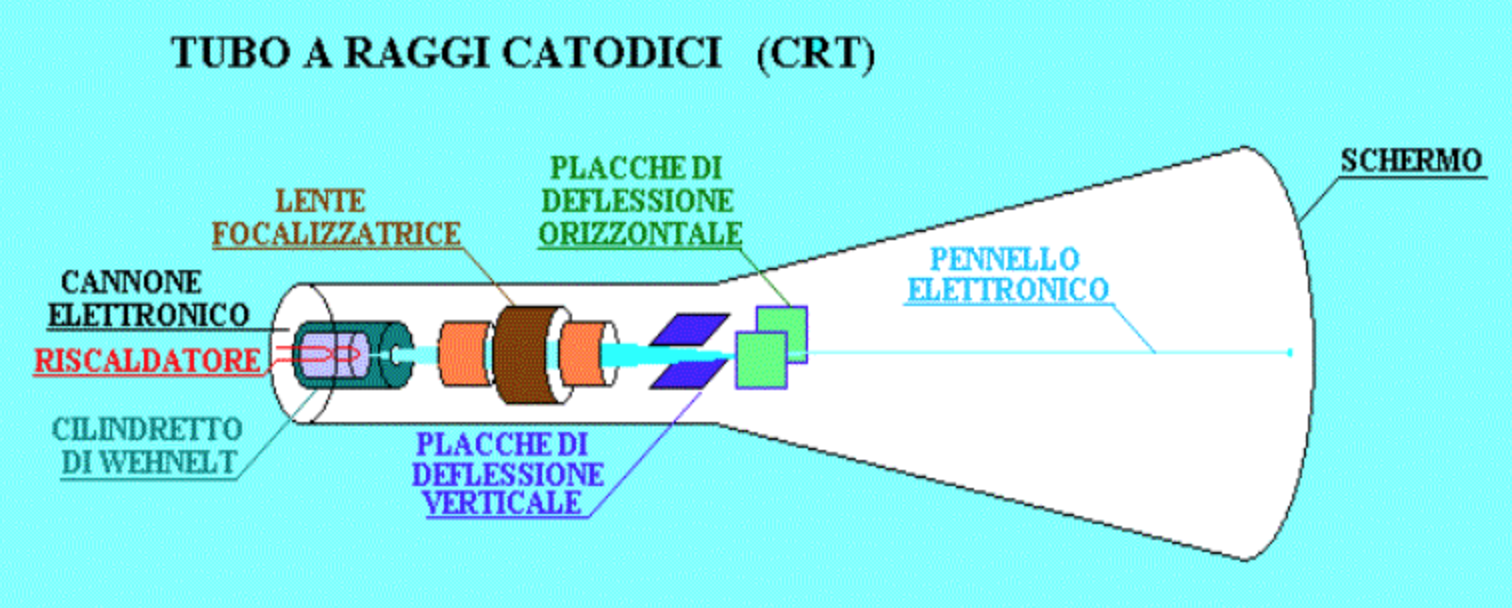
\includegraphics[width=\textwidth]{images/osc_analog.png}
  \caption{Schema a blocchi Oscilloscopio Analogico}
  \label{fig:osc_analog}
\end{figure}

L'avvento del \textbf{digitale} ha portato sicuramente a notevoli vantaggi, il nuovo strumento, \textit{oscilloscopio digitale}, si presenta, a livello funzionale, identico al precedente con molte funzioni aggiunte a livello matematico, ecc... Ma con importanti differenze strutturali infatti il segnale dopo essere stato trasdotto verrà campionato (cap. \ref{d1}), convertito, memorizzato ed infine visualizzato.\\
L'intero strumento demanda tutte le operazioni di gestione e calcolo alla sua CPU interna per poi visualizzare il segnale in questione su un display non più a fosfori ma con semplici pixel (tubi raster).
\paragraph{Acquisizione} Questa fase è fondamentale per la corretta rappresentazione del segnale infatti esso dovrà essere quantizzato, ovvero rappresentato con un numero finito di bit (introducendo anche un'errore). Una volta tradotto dovrà essere memorizzato in apposite memorie (SSD) che verranno gestite come buffer circolari.
\paragraph{Campionamento} Verrà analizzato meglio nel capitolo \ref{d1} ma si tratta della procedura necessaria a tradurre un segnale da analogico a digitale. Questo processo, a patto che venga rispettato il teorema di Shannon, non introduce perdite.
\paragraph{Aliasing} Esso è un fenomeno direttamente correlato al campionamento infatti esso introduce una periodicizzazione dello spettro del segnale, con periodo pari alla frequenza di campionamento $F_{C}$. Fin tanto che $F_{C}>2B$ non abbiamo sovrapposizione di questi alias e possiamo tranquillamente separarli tramite un filtro passa basso (figura \ref{fig:si_fc}). Se invece questa condizione non viene rispettata gli alias si sovrapporranno portando ad uno spettro da cui non sarà più possibile ricostruire il segnale originario (figura \ref{fig:no_fc}).

\begin{figure}[!hpt]
  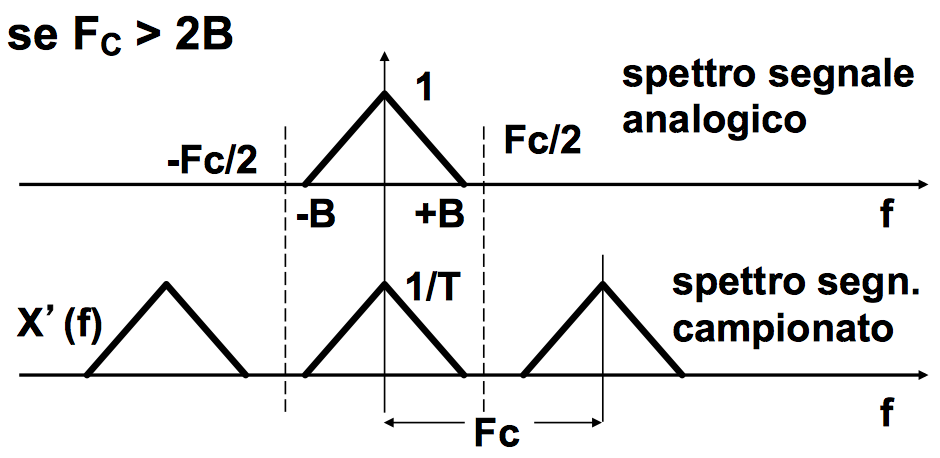
\includegraphics[width=\textwidth]{images/si_fc.png}
  \caption{Teorema di Shannon rispettato}
  \label{fig:si_fc}
  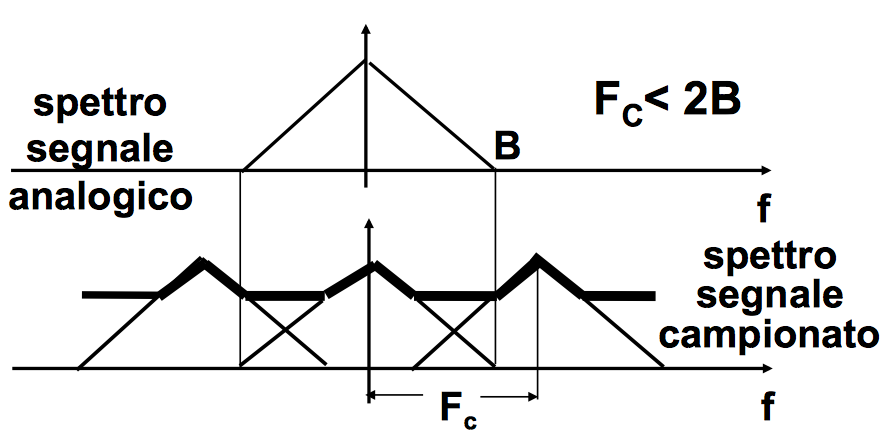
\includegraphics[width=\textwidth]{images/no_fc.png}
  \caption{Teorema di Shannon NON rispettato}
  \label{fig:no_fc}
\end{figure}

\paragraph{Sequential/Random Sampling} E' un procedura con la quale il convertitore viene comando per campionare il segnale con ritardi crescenti rispetto all'istante di trigger, spesso viene anche realizzato mediante campionamento casuale. Sul pannello verrà visualizzato:
\begin{itemize}
  \item \textbf{ONE-SHOT}: Segnali transitori.
  \item \textbf{NORMAL}: Segnali periodici o ripetitivi.
\end{itemize}

\paragraph{Altre opzioni del DSO} L'oscilloscopio digitale permette molte altre funzioni come:
\begin{itemize}
  \item Visualizzazione:
  \begin{itemize}
    \item \textbf{Average}: Media su più tracce
    \item \textbf{Peak o Envelope}: Massimo e minimo per una serie di tracce
    \item \textbf{Cumulative}: Mostre tutte le tracce senza ripulire il display
  \end{itemize}
  \item Misura:
  \begin{itemize}
    \item \textbf{FFT}
    \item \textbf{Cursori}: sia asse tempi che asse tensioni
    \item altro: Rise, fall, freuqnza, periodo, sfasamento, ecc...
  \end{itemize}
\end{itemize}

Altra cararatteristica importate è la possibilità di utilizzare lo strumento in multicanale, il problema dell'acquisizione da più canali può essere risolto o con più memorie o con velocità doppia.

\paragraph{Trigger} Durante il quotidiano utilizzo di un'oscilloscopio avremo a che fare con l'istante di trigger, con il vecchio oscilloscopio le uniche opzioni riguardavano il \textbf{livello}, la \textbf{pendenza} e sempre in \textbf{post-trigger}. Con lo strumento digitale invece il numero di opzioni aumenta enormemente, possiamo settare, oltre ai valori standar, anche trigger a due livelli (con isteresi), trigger a più canali, trigger da pattern, trigger automatici, ecc...

\paragraph{Visualizzazione} Il numero di pixel disponibili sullo schermo è pari a $N_{V}$, mentre la memoria di acquisizione contiene $N_{I}$ campioni, va da se che ne il numero di campioni è maggiore del numero di pixel allora dovrò effettuare un ``selezione'' dei dati da visualizzare, se invece si presenta la situazione opposta sarà necessario gestirlo in modo appropriato.\\
Nel caso di segnale $N_{I}<N_{V}$ le opzioni sono due, o visualizzo i campioni che effettivamente ho (modalità dot), oppure adotto un'algoritmo di interpolazione, illustrati nel successivo paragrafo, in modo da aver un numero di punti accettabile a visualizzare correttamente la traccia. Ovviamente il teorema di Shannon dovrà essere rispettato ($F_{EV}>2F_{S}$), se il rapporto dei due fattori risulta essere:
\begin{itemize}
  \item \textbf{Irrazionale}: Immagine confusa con campioni distribuiti in modo casuale.
  \item \textbf{Razionale}: Nessuna SENSAZIONE di errore, forma d'onda correttamente vista, ampiezza coretta ma frequenza notevolmente diversa.
\end{itemize}
Da queste considerazioni derivano poi fenomeni come l'\textbf{aliasing percettivo} (il sistema di percezione visivo umano interpola in modo errato ciò che vede, figura \ref{fig:alias_perc}).

\begin{figure}[!hpt]
  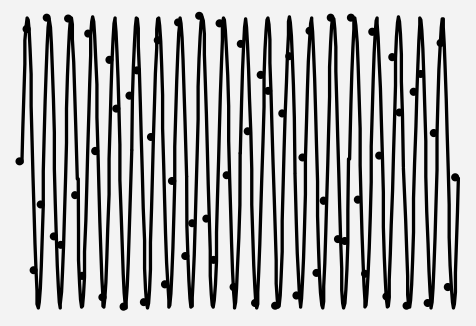
\includegraphics[width=\textwidth]{images/alias_perc.png}
  \caption{Esempio di aliasing percettivo}
  \label{fig:alias_perc}
\end{figure}
Una corretta visualizzazione richiede almeno 20-25 punti per periodo.

\paragraph{Interpolazione} Nel caso in cui non ci siano sufficenti campioni per la visualizzazione dobbiamo occuparci di interpolare al meglio in nostri campioni in modo da generare un segnale utilizzabile sul nostro display.\\
Nel caso di \textbf{interpolazione lineare} sono necessari circa una decina ci punti, questo algoritmo potrebbe comunque portare ad errori grossolani.\\
Parlando invece di \textbf{interpolazione Sinc} si utilizza una sommatoria infinita (dove i campioni più lontani hanno peso praticamente nullo) che permette una miglior approssimazione della curva, introducendo però problemi quali il fenomeno di Gibbs o fronti poco accurati.\\
Sono disponibili altre tecniche che non verranno studiate, generalmente non viene reso disponibile all'utente final l'algoritmo di interpolazione.

\paragraph{Specifiche DSO} Altre informazioni utili possono essere:
\begin{itemize}
  \item Bit equivalenti: Tutte le cause di errore introdotte dal convertitore A/D ideale con bit inferiori a quello reale.
  \item Banda passante: Spesso riportate per one-shot e casuale costituiscono la banda di frequenza accettabile dallo strumento.
  \item Frequenza di campionamento: Anche qui divisa in repetitive e one shot, espressa in Sample al secondo.
  \item Accuratezza verticale: Come parametro unico o formula binomia.
\end{itemize}

\paragraph{Sonde} Le sonde sono gli strumenti attraverso i quali connettiamo i segnali al nostro strumento, spesso sono costituite da un cavo coassiale per essere connesse al terminale BNC. Le classiche sonde hanno una resistenza di ingresso elevata per ridurre l'effetto del carico ma la loro reattanza capacitiva introduce comunque una variazione nel segnale. Con l'utilizzo delle \textbf{sonde compensate} invece si riesce, routando direttamente una vite azionante il circuito di compensazione, a variare il polo introdotto dalla sonda in modo da rendere indipendente il segnale dalla frequenza.



% Parte B
\section{Parte B}
% PARTE B1 - ELAPMISB1
\subsection{Parte B1}\label{b1}
I circuiti logici digitali sono caratterizzati da una tensione di alimentazione che varia dal GND a Val. I segnali di ingresso possono essere ricevuti in modo seriale o parallelo.\\
Gli stati logici di uscita sono rappresentati da tensioni, solitamente la tensione alta ($V_{al}$) corrisponde al valore logico 1 e prende il nome di $V_{h}$, mentre la tensione bassa (GND) corrisponde al valore logico 0 e prende il nome di $V_{l}$.\\

\begin{wrapfigure}{R}{0.38\textwidth}
  \centering
  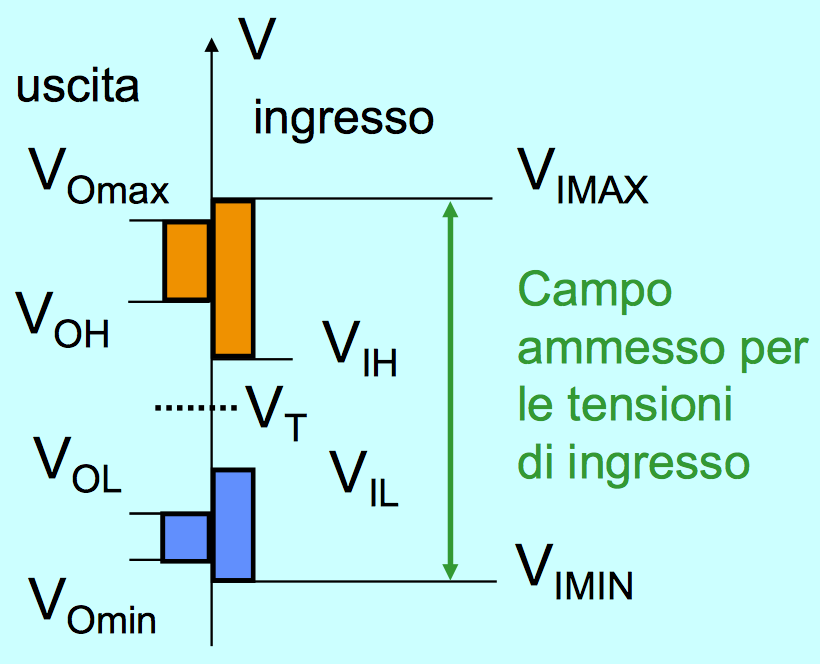
\includegraphics[width=0.35\textwidth]{images/compat.png}
  \caption{Compatibilità tra porte logiche}
  \label{fig:compat}
\end{wrapfigure}

La capacità di riconoscimento dell’ingresso da parte di una porta logica è legata al confronto con una soglia. Per poter garantire il corretto funzionamento di un circuito vengono specificati dei campi di accettabilità degli ingressi. Se essi vengono rispettati ($V_{ol}$ $<$ $V_{il}$ e $V_{oh}$ $>$ $V_{ih}$) la dall’uscita precedente allora non vi saranno problemi di compatibilità tra le porte questo è infatti il principale vantaggio del mondo digitale, usando un semplice comparatore di soglia siamo in grado di rigenerare il segnale alla perfezione. I margini di rumore sono le fasce dove il segnale di entrata potrà ancora essere riconosciuto correttamente, esse sono commisurate al tipo di applicazione del circuito, le auto avranno NM molto ampi. Una rappresentazione grafica della compatibilità si può vedere in figura \ref{fig:compat}

\paragraph{Transistor} I circuiti di tipo CMOS (MOS complementari) hanno una diversa resistenza di uscita nel caso in cui si parli di uscita alta o bassa, anche la tensione di uscita Vo è consistente solo in base ai valori di Io. Questo tipo di circuiti prevede solamente due tipi di uscita H o L. Nel circuito a tre stati abbiamo anche l’opzione Z = alta impedenza utile in casi in cui all’uscita non si voglia avere ne un valore H ne un valore L, questo tipo di circuito può essere implementato anche con un doppio switch. Molto considerazioni fatte tralasciano il fattore realtà infatti dobbiamo tenere in considerazione alcuni fattori. I segnali reali hanno fronti con pendenza finita e quindi il riconoscimento del nuovo stato logico non è immediato, allo stesso modo anche le variazioni di tensioni o correnti nei moduli stessi non lo possono essere. La combinazione di tutti questi parametri limita la velocità di operatività e porta a ritardi di propagazione.\\
Il tempo di propagazione è il tempo necessario, per un segnale in ingresso a propagarsi nel modulo fino alla sua uscita. Questo valore non sempre è uguale per le due transizioni, lo è nel caso di strutture simmetriche come i CMOS, non lo è nel caso di uscita R-SW (dove abbiamo un transitorio in carica molto lento). Il FAN OUT rappresenta il massimo numero di ingressi che possono essere collegati ad una uscita.
\paragraph{Segnali Differenziali} I segnali differenziali hanno numerosi vantaggi in quanto sono protetti dai disturbi, o meglio essendo un doppia canale tutti e due vengono disturbati allo stesso modo mantenendo così il valore differenziale uguale. Ci permettono inoltre di usare una differenza di tensione molto più bassa aumentando così la velocità e riducendo i consumi.

% PARTE B2 - ELAPMISB2
\subsection{Parte B2}\label{b2}
I circuiti combinatori sono funzioni combinatorie degli ingressi applicati e non hanno bisongno di elementi di memoria a differenza dei circuiti sequenziali i quali sono funzioni anche della precedente storia del circuito.

\paragraph{Elementi di memoria} Il primo elemento di memoria è l'anello di inverter ma il suo svantaggio è legato al fatto che una volta assegnatoli in valore non è possibile modificarlo senza rimuovere l'alimentazione. Altra questione di interesse in questo elemento è legata alla situazione di metastabilità (stato temporaneo intermedio) da evitare. Da questo si passa subito al FF Set Reset. Esso presenta l'anello di inverte con due porte NOR che fungono da commutatori nel circuito. Le situazioni possibili sono 4 modificando in modo complementare SET e RESET si modifica il valore, con SET a 1 Qa=1 ecc... Nel caso in cui tutti e due i comandi siano a 0 si crea l'anello di inverter, entrando in stato di memoria. L'ultima condizione (TUTTI 1) è una situazioni proibita dove rischio di mandare in stallo (uscite uguali o metastabilità) il sistema. Una possibile soluzione al problema dello stallo è quella di assegnare i comando S ed R allo stesso segnale opportunamente invertito in un caso. Il sistema può essere volendo convertito (legge di De Morgan) con porte NAND.

\paragraph{Sync o Async} I Circuiti possono essere sincroni o asincroni, i primi sono molto più semplici da realizzare (CAD Automatici) e possono cambiare il loro stato solo in presenza di un comando specifico (CLK). Viene aggiunto un segnali di crontrollo LE (Latch Enabled) per controllare le situazioni in cui può effettivamente variare lo stato.\\
I FF Master-Slave sono costituiti da una cascata di FF latch con abilitazione complementare su base CLK, se =0 abilito il primo e blocco il secondo, mentre se =1 l'opposto.\\
Riepilogo:
\begin{itemize}
  \item Latch: (Attivo su livello)
  \begin{itemize}
    \item \textbf{LE = 1} Trasparenza
    \item \textbf{LE = 0} Memoria
  \end{itemize}
  \item FF D (Master-Slave): (Attivo su fronte)
  \begin{itemize}
    \item Uscita variante su fronti del CLK
    \item Non fronte = Memoria
  \end{itemize}
\end{itemize}
FF JK è basato su un SR MS con reazione incrociata, la principale differenza è legata alla sua possibilità di sfruttare la situazione normalmente proibita.\\
Tutti questi cricuiti essendo reali presentano non idealità dovute principalmente ai ritardi di propagazione dei segnali. Bisogna quindi tenere in considerazione anche queste cose (La frequenza di CLK viene determianta sulla base di questi ritardi).\\
I principali sono:
\begin{itemize}
  \item \textbf{Tsetup} = Minimo tempo necessario tra il cambio di stato di D ed ilrise del CLK.
  \item \textbf{Trise} = Tempo di salita del fronte di CLK.
  \item \textbf{Thold} = Minimo tempo necessario dopo il rise del clock, ma prima del successivo cambio di stato.
  \item \textbf{Tfall} = Tempo di discesa del fronte di CLK.
\end{itemize}
In figura \ref{fig:timingdff} una rappresentazione completa del timing di un D-FF.
\begin{figure}[!hp]
  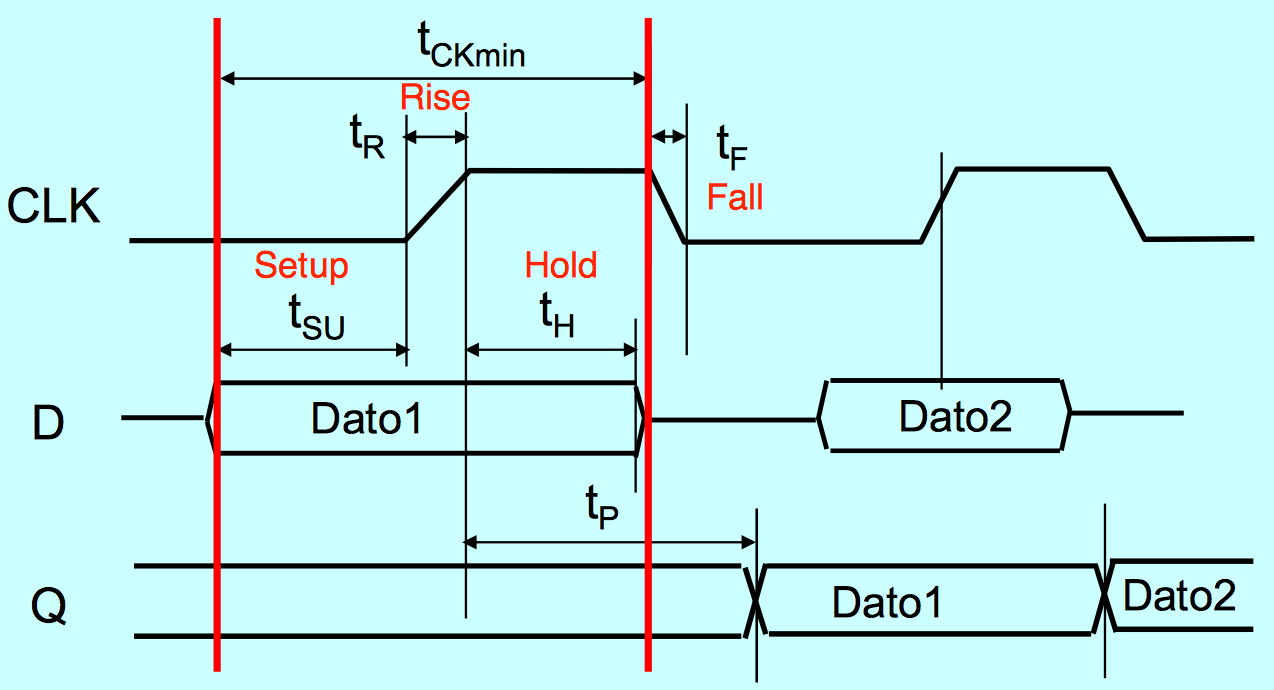
\includegraphics[width=\textwidth]{images/timingdff.png}
  \caption{Timing completo di un D-FF}
  \label{fig:timingdff}
\end{figure}

% PARTE B3 - ELAPMISB3
\subsection{Parte B3}\label{b3}
I segnali possono essere trattati in due forme, seriale o parallela.\\
Nel trasferiemento seriale uno alla volta i segnali vengono cadenzati da un segnale di CLK (1 bit x volta). In quello parallelo invece vengono trasferiti N bit per volta in un singolo segnale di CLK. Potrebbe sembrare che la seconda sia sempre più veloce, nella realtà potendo sfruttare una frequenza decisamente alta le connessioni seriali sono più veloci (vedi USB).

\paragraph{Registri} I registri sono le componenti grazie alle quali possiamo mantenere i dati. Essi sono costituiti semplicemente da FF uniti di tipo L o Edge-Triggered dove viene utilizzata una sola uscita. Vi sono differenti tipi di registri:
\begin{itemize}
  \item \textbf{PIPO}: Parallel In / Parallel Out
  \item \textbf{Shift-Register}: Serial In / Serial Out
  \item \textbf{SIPO}: Serial In / Parallel Out
  \item \textbf{PISO}: Parallel In / Serial Out
\end{itemize}

\paragraph{Contatori} Circuiti logici in grado di generare sulle uscite una sequenza di conteggio binario incrementata ad ogni colpo di CLK. Possono essere si crescenti che decrescenti.\\
I divisori invece sono costituiti da FF in cascata dove l'uscita di uno diventa il CLK del successivo. Questo permette di modulare (dividere) la frequenza di CLK. Chiaramente in tutti questi componenti non possiamo trascurare la questione ritardi. Se usiamo contatori sincroni il ritardo non sarà nullo, ma semplicemente sarà uguale per tutte le componenti facendole rimanere sincronizzate. Nel caso di CLK concatenato tra le porte la questione sarà molto più difficile da gestire andato di fatto a generare un circuito asincrono. In qualsiasi caso valgono tutte le regole di sincronizzazione.

\paragraph{Temporizzazione} Nel calcolare la massima frequenza di operatività del circuito devo tenere in considerazione molte variabili:
\begin{itemize}
  \item Ritardo introdotto dal FF (Uscita dalla porta del segnale entrato).
  \item Ritardi introdotti dalla logica combinatoria (porte AND in questo caso).
  \item Tempo di SETUP richiesto dal FF.
\end{itemize}
Per poter ridurre i ritardi in questione non mi conviene usare strutture a riporto (Ripple) ma quelle dirette (Look Ahead) che mi permettono di risolvere tutti i problemi dovuti alla logica combinatoria. Il principale svantaggio di queste strutture è legato alla complessita di progettazione.

% PARTE B4 - ELAPMISB4
\subsection{Parte B4}\label{b4}
I comparatori di soglia sono elementi fondamentali nell'elettronica digitale, il primissimo compito è quello di pulizia dei segnali (vedi figura \ref{fig:comparator}) in modo da riportarli al loro valore privo di disturbi.
\begin{figure}[!hp]
  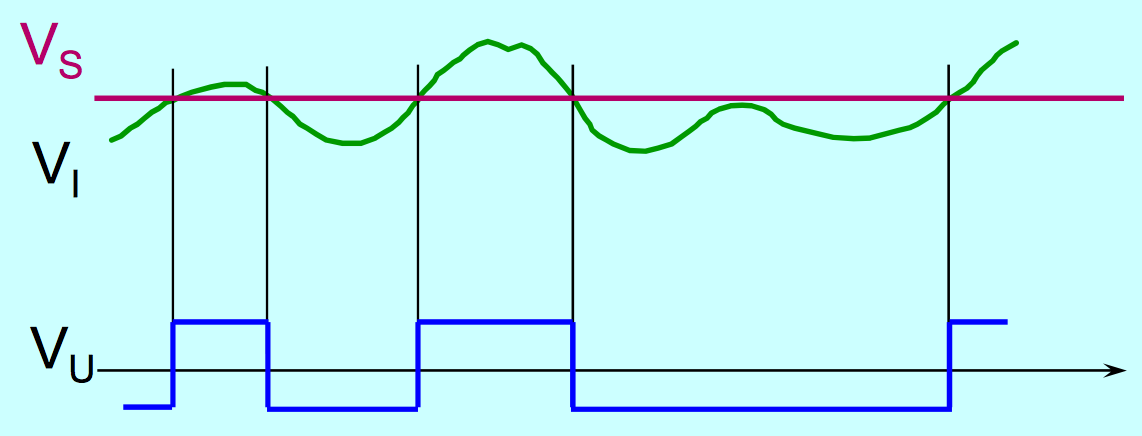
\includegraphics[width=\textwidth]{images/comparator.png}
  \caption{Comparatore non invertente}
  \label{fig:comparator}
\end{figure}

\paragraph{Comparatori con A.O.} Questo tipo di comparatori presenta alcune controindicazioni dovute a:
\begin{itemize}
  \item Guadagno \textbf{Ad} ad anello aperto molto grande.
  \item Escursione della \textbf{Vu} limitata.
  \item Zona lineare molto ridotta.
\end{itemize}
Il comparatore può essere realizzato sia con AO invertente che non, con una semplice inversione del segnale di uscita. Il problema principale di questa soluzione, con una sola soglia di confronto, è che un segnale "rumoroso" potrebbe creare un'uscita pessima con tantissimi cambi di valore.\\
In queste situazioni:
\begin{itemize}
  \item Fuori linearità.
  \item Elevata tensione differenziale tra gli ingressi.
  \item Eventuale tensione di modo comune.
\end{itemize}

\paragraph{Comparatore con Isteresi} La differenza principale è legata all'utilizzo di due soglie invece che una singola, questo permette di avere un sistema più resistente al rumore infatti il valore di uscita commuterà solo al passaggio della soglia più esterna. Questa è un sistema con isteresi. Anche questa soluzione può essere implementata con tutti e due i tipi di AO. Per ottenere uno sdoppiamento della soglia è sufficente creare un partitore di tensione (utilizzando resistenze) tra l'uscita ed una tensione di riferimento.

\paragraph{Comparatori Integrati} Esistono componenti più specifici con uscite più flessibili, maggiore velocità o non idealità meno importanti. Uno di questi è il trigger di Schmitt con soglie fisse e inverter con ingresso a trigger. Il circuito è semplice, un condensatore a massa, componente e resistenza in parallelo e si misura la tensione di uscita rispetto a GND.

\paragraph{Convertitori} Il comparatore di sogli trasforma una grandezza analogica in una numerica (su 1 bit). In generale per convertire un segnale A/D avremo bisongo un numeri di comparatori $2^n-1$ (n: numero di bit). Eventualmente si possono conbinare comparatori in cascata.

% PARTE B5 - ELAPMISB5
\subsection{Parte B5}\label{b5}
Gli oscillatori ed i generatori di segnali sono utili strumenti nel campo dell'elettronica.

\paragraph{Generatori di Segnali} Ci possono essere diversi tipi di generatori di segnali, continui o ad impulsi.\\
I principali parametri da tenere in considerazione in un segnale, a seconda del tipo sono:
\begin{itemize}
  \item Livelli: $V_{H}, V_{L}$
  \item Periodo: $T = T_{H} + T_{L}$
  \item Frequenza: $1/T$
  \item Duty Cycle: $DC = T_{H}/T$
  \item Ampienzza: A
\end{itemize}
Il generatore di onda quadra generale un segnale rettangolare con DC specificato. Il generatore di impulso è un circuito monostabile generante un singolo impulso di larghezza W.\\
I vari segnali possono essere ritardati, per farlo possono essere usate diverse soluzioni, nei circuiti analogici con celle RC o LRC. Nei circuiti digitali con contatori, o soluzioni ad hoc. Con il software la soluzione è molto più semplice. Spesso si farà uso della celle RC di cui si riporta uno schema in figura \ref{fig:rc}
\begin{figure}[!hp]
  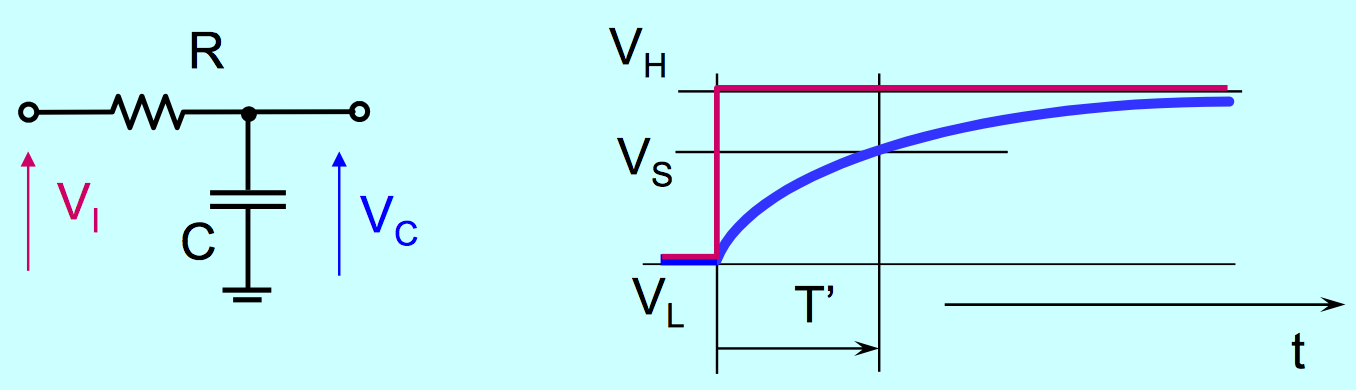
\includegraphics[width=\textwidth]{images/cellRC.png}
  \caption{Cella RC}
  \label{fig:rc}
\end{figure}
Si riporta anche la formula per calcolare il tempo di raggiungimento della soglia:\\
\begin{equation}
  \begin{gathered}
    T' = -RC\cdot ln\frac {(V_{H}-V_{S})} {(V_{H}-V_{L})}
    \label{eq:tsoglie}
  \end{gathered}
\end{equation}

\paragraph{Generatori di Onda Quadra} Il segnale O.Q. può essere ottenuto concatenando due parti: una rete RC passa-basso comandata da un segnale BINARIO sfruttando la carica e scarica del condensatore, un comparatore con isteresi. Se il comparatore pilota la rete RC otteniamo proprio un onda quadra in quanto il nostro condensatore si caricherà e scaricherà tra le due soglie ($V_{S1}, V_{S2}$).\\
I principali limiti operativi sono legati alla resistenza di reazione. Con una grande resistenza non riusciremo a far circolare la corrente necessaria, valori troppo bassi invece limitano la dinamica di uscita. Allo stesso modo il condensatore non deve avere un valore troppo basso altrimenti introdurrebbe una capacità parassita.\\
In modo analogo è possibile ottenre un generatoe di onda triangolare.\\
Il valore del periodo: $T_{1} = (R*C*(V_{S2}-V_{S1}))/V_{UH}$ è modificabile variando il valore della resistenza di reazione. La variazione di DC è più complessa e necessità dell'utilizzo di due diodi.\\

\paragraph{Oscillatori sinusoidali} Per realizzare questo componente spesso vengono utilizzati quarzi o altri materiali piezoelettrici in grado di deformarsi in presenza di un campo elettrico o di generare tensione se sottoposti a sollecitazioni meccaniche. Altra possibile soluzione è sfruttando circuiti con reazione, reti RC e porte.

% PARTE B6 - ELAPMISB6
\subsection{Parte B6}\label{b6}
Ad oggi l'industria elettronica non si occupa della produzione di un'oggetto nella sua interezza, si utilizzano componenti costruiti da altre aziende principalmente perchè ridurre il tempo di progettoed abbassare i NRE Cost (Non-Recurrent Engineering Cost). Le problematiche legate a questa soluzione sono correlate alla più difficile comprensione delle componenti (datasheet complessi). In generale ci sono 3 tipi di industrie:
\begin{itemize}
  \item Progetto di \textbf{Sistemi} (Nokia, Apple, Marelli, ...)
  \begin{itemize}
    \item Possono includere la produzione.
    \item Poco specializzate, molte migliaia di aziende.
  \end{itemize}
  \item Progetto di \textbf{Circuiti integrali} (Intel, Texas Instruments, ...)
  \begin{itemize}
    \item Produzione quasi assente.
    \item Specializzate nella produzione di maschere per i CI.
  \end{itemize}
  \item Fabbricazione di \textbf{Circuiti Integrati} (Intel, Samsung, TSMC, ...)
  \begin{itemize}
    \item Molto specializzate, meno di 10 al mondo, per gli altissimi costi di ammortamento degli impianti.
  \end{itemize}
\end{itemize}

\paragraph{Tempo di progetto}
 l tempo di progetto è fondamentale, il ritardo di ingresso si trasferisce quadraticamente sui ricavi.
\paragraph{Costi} I contribuenti al costro per prodotto sono molti: NRE (una tantum), Cu (costo unitario di produzione escludente i costi di progetto).\\
$C_{p} = (NRE/N) + Cu$\\
Le diverse scelte dipendono principalmente dal numero di unità prodotte N.

\paragraph{Stili di progetto} Vi possono essere differenti stili dai quali dipenderanno molto i costi. Si può partire costruenti circuiti direttamente con le porte fino ad arrivare ad HW generico sfruttante funzioni definite lato SW.
\begin{itemize}
  \item \textbf{FULL CUSTOM}: Necessitano moltissimi step progettuali con altissima flessibilità, il tutto altissimi NRE cost.
  \item \textbf{SEMI CUSTOM}: Sfruttano librerie di progetto, rimangono comunque complessi da sviluppare garantendo una discreta flessibilità ma comunque con alti costi.
  \item \textbf{Cir. Programmabili}: Presentano IN/OUT programmabili, senza nessuna funzione nativa ma con bassi NRE ed alti costi unitari.
\end{itemize}

\paragraph{Logiche Programmabili} La semplicitià di queste componenti le rende molto diffuse e di facile utilizzo. La loro struttura è basata su matrici di IN/OUT dove i collegamenti risultano definibili dagli utenti. Le principali logiche sono PAL o PLA. Altri tipi di memorie programmabili sono PROM (eventualmente a sola lettura come nei computer), FPGA (complesse fino a decine di milioni di porte), EEPROM (basate su MOS floating gate).

% PARTE C
\section{Parte C}
% PARTE C1 - ELAPMISC1
\subsection{Parte C1}\label{c1}
Le tecnologie attuali permettono di avere un numero di transisto $>10^9$ per chip (Intel i7). Il principale bottle neck rimanere la distribuzione dei segnali e l'energia. I circuiti usano simboli binari, ma nella realtà sono tensioni e correnti.

\paragraph{Ritardi} Tenendo in considerazioni tutte le questioni legate all'interfacciamento delle componenti viste nella parte B andiamo a considerare ulteriori imprecisioni. Le più importanti sono il Clock Jitter $T_{J}$ (variazione $\pm$ del periodo) ed il Clock Skew $T_{K}$ (sfasamento $\pm$ tra clock).

\paragraph{Interconnessioni} A livello ideali l'uscita logica del driver (TX) e l'ingresso logico del receiver (RX) presentano una connessione perfetta, senza ritardi e disturbi, chiaramente solo in prima approssimazione.\\
Se cerchiamo di ottenere una più precisa approssimazione dobbiamo andare ad analizzare il circuito come una linea di comunicazione dopo il collegamente D-R viene modellato come una cella RC passa-basso. Conseguentemente, al segnale in uscita dal driver avremo una risposta esponenziale con costante di tempo $\tau = CR$. Il ritardo con cui viene rilevata una variazione di stato logico prende il nome di TEMPO DI TRASMISSIONE ($t_{TX}$). Questo tempo varia anche tra connessioni nominalmente allinetate e la differenza tra i due casi ($t_{TXmax}-t_{TXmin}$) prende il nome di SKEW.

\begin{figure}[!hp]
  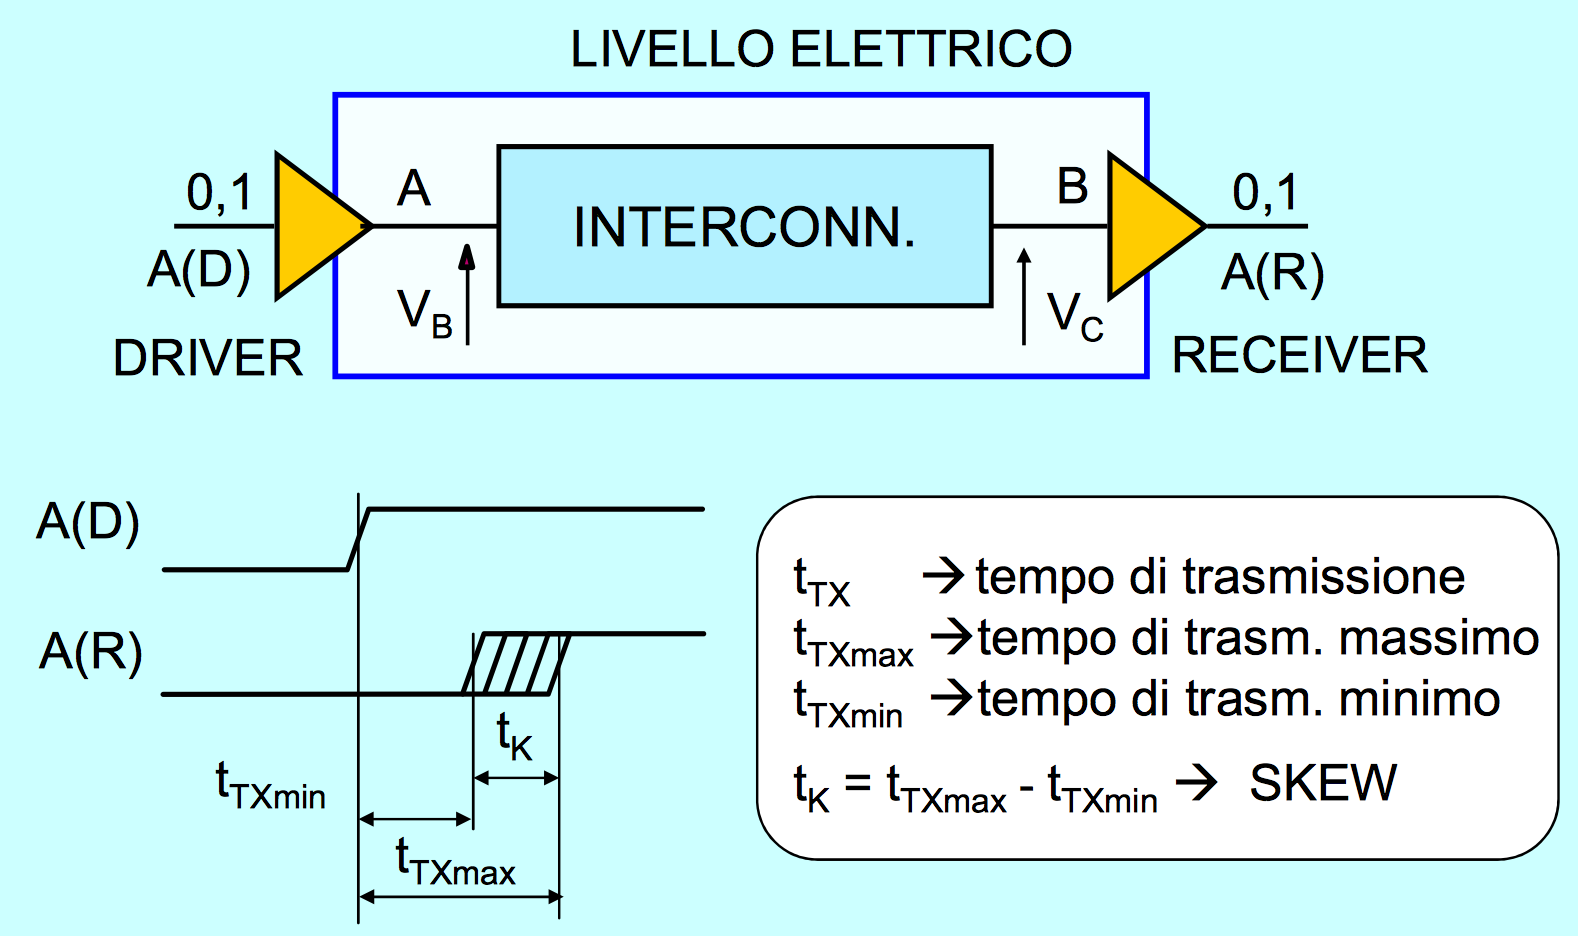
\includegraphics[width=\textwidth]{images/interc.png}
  \caption{Parametri di interconnessione}
  \label{fig:interc}
\end{figure}

% PARTE C2 - ELAPMISC2
\subsection{Parte C2}\label{c2}
L'approssimazione con celle RC è discretamente valida, vi sono anche le approssimazioni a parametri concentrati. Idealmente aumentando il numero di celle ad infinito si ottiene una linea di trasmissione reale.\\
Ogni linea presenta dei parametri caratteristici:
\begin{itemize}
  \item Parametri Fisici:
  \begin{itemize}
    \item Lu: Impedenza unitaria
    \item Cu: Capacità unitaria
  \end{itemize}
  \item Parametri Elettrici:
  \begin{itemize}
    \item Impedenza caratteristica: $Z_{\infty}$ (10...1000 $\Omega$)
    \item Velocità di propagazione: P=(0.6-0.8)*C
    \item Tempo di propagazione: (tempo di spostamento sul conduttore) $t_{p}=L/P$
  \end{itemize}
\end{itemize}

\paragraph{Linea Pilotata} Il primo gradino si sposta lungo tutto il conduttore senza subire distorsioni ed impiega un $t_{p}$ a propagarsi fino all'ingresso del receiver su una linea senza perdite.\\
Se $R_{t}=Z_{\infty}$ allora in rapport $V/I$ non varia e non si hanno discontinuità. Se invece $R_{t} \neq Z_{\infty}$ il rapporto $V/I$ varia, generando una progressiva variazione del gradino (onda progressiva o incidente), le variazioni genereranno un'onda riflessa (regressiva) con propagazione inversa a prima.\\
L'ampiezza dell'onda riflessa sarà determinata dal coefficente di riflessione $\Gamma_{T}$ con $V_{r}=\Gamma_{T}V_{p}$.\\
Questo coefficente assume valori differenti:
\begin{itemize}
  \item \textbf{Linea Chiusa}: $R_{t}=Z_{\infty}$ allora $\Gamma_{T}=0$
  \item \textbf{Linea Aperta}: $R_{t}\rightarrow\infty$ allora $\Gamma_{T}=1$
  \item \textbf{Linea in Corto}: $R_{t}=0$ allora $\Gamma_{T}=-1$
\end{itemize}
L'andamento del sistema viene spesso schematizzato utilizzando un diagramma a traliccio (vedi figura \ref{fig:tralicc}). In tutto questo dobbiamo ricordare che le variazioni di stato logico sono riconosciute quando viene attraversata la soglia $V_{TH}$; questo può richiedere riflessioni multiple del segnale, e introduce un ritardo $t_{TX}$ (tempo di trasmissione) tra attivazione del segnale e la rilevazione della variazione al ricevitore.

\begin{figure}[!hp]
  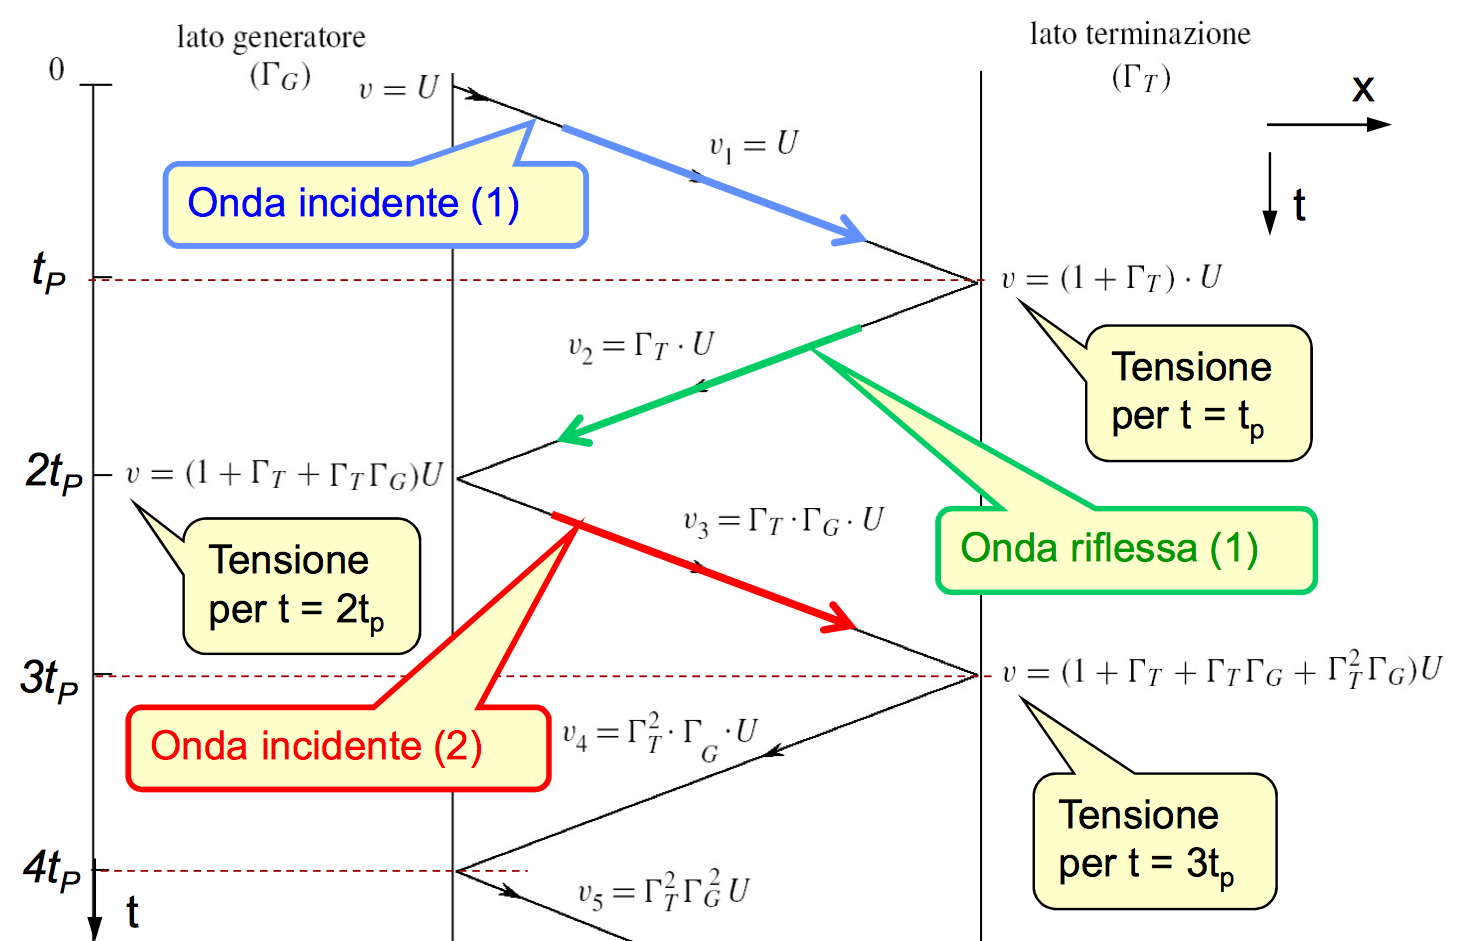
\includegraphics[width=\textwidth]{images/tralicc.png}
  \caption{Diagramma a traliccio}
  \label{fig:tralicc}
\end{figure}

Per calcolare il primo gradino si utilizza la formula:
\begin{equation}
  \begin{gathered}
    V_{B}(0)=\frac{Z_{\infty}}{R_{O}+Z_{\infty}}V_{A}=V_{1}
    \label{eq:veff}
  \end{gathered}
\end{equation}

% PARTE C3 - ELAPMISC3
\subsection{Parte C3}\label{c3} % 15 Dicembre 2016
Il tempo di trasmissione $t_{TX}$, il ritardo di attraversamento della soglia, dipende da molti parametri. Le variazioni di $t_{TX}$ portano allo skew $t_{K}$ o disallineamento.

\paragraph{skew} Diretta conseguenza è la modifica delle relazioni temporali tra i segnali. E' importante riusire a gestirlo in modo da preservare l'integrità dei segnali. I principali contribuenti a questo paramentro sono:
\begin{itemize}
  \item Prametri TX ed RX ($V_{H}$, $V_{L}$, soglie, ecc...)
  \item Propagazione: riflessioni, terminazioni, discontinuità, diafonia, ecc...
  \item Carico (in particolare capacitivi)
  \item Rumore di massa (Ground Bounce) e di commutazione
\end{itemize} %18 Dicembre 2016
\paragraph{Tipi di commutazione} Il tipo di commutazione della nostra linea dal rapporto $R_{O}/Z_{\infty}$ oppure dal tipo di corrente:
\begin{itemize}
  \item \textbf{BASSO Rapporto} $R_{O}<Z_{\infty}$: $\rightarrow$ I gradino ampio.\\ La soglia viene attraversata, commutazione su onda incidente (IWS), basso $t_{TX}$ e veloce. Richiede terminazione (adatto a BUS). Vedi figura \ref{fig:iws}
  \item \textbf{ALTO Rapporto} $R_{O}>Z_{\infty}$: $\rightarrow$ I gradino basso.\\ Soglia non attraversata, commutazione su onda riflessa (RWS), alto $t_{TX}$ e lento. Non sono necessarie terminazione (adatto per sistemi lenti). Vedi figura \ref{fig:rws}
  \item \textbf{BASSA Corrente}, con $R_{O}$ alta, la soglia viene attraversata dopo riflessioni multiple (vedi figura \ref{fig:att_mult}) con un funzionamento lento.
\end{itemize}

\begin{figure}[!hp]
  \centering
  \begin{minipage}{.3\textwidth}
    \centering
    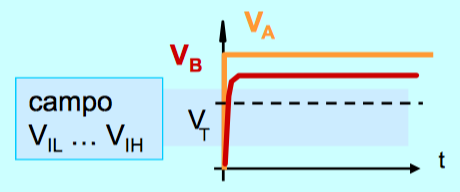
\includegraphics[width=\linewidth]{images/iws.png}
    \caption{IWS}
    \label{fig:iws}
  \end{minipage}\hfill
  \begin{minipage}{.3\textwidth}
    \centering
    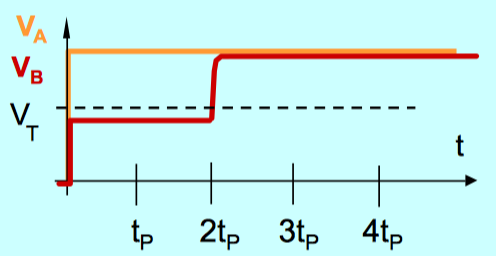
\includegraphics[width=\linewidth]{images/rws.png}
    \caption{RWS}
    \label{fig:rws}
  \end{minipage}\hfill
  \begin{minipage}{.3\textwidth}
    \centering
    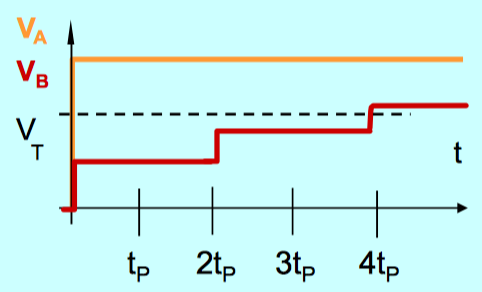
\includegraphics[width=\linewidth]{images/att_mult.png}
    \caption{Attr. Multiplo}
    \label{fig:att_mult}
  \end{minipage}
\end{figure}

% PARTE C4 - ELAPMISC4
\subsection{Parte C4}\label{c4}
Le operazioni a livello ciclo hanno lo scopo di garantire il corretto trasferimento delle informazioni trasferite dal livello fisico. La temporizzazione di un sistema non è banale, spesos i ritardi sono funzioni del tempo, difficili quindi da prevedere con esattezza.
\paragraph{Trasferimento Informazioni} Vi sono due tipi di trasferimento dei dati:
\begin{itemize}
  \item Attivato dalla \textbf{sorgente} $\rightarrow$ Scrittura. Direzione controllo = informazione.
  \item Attivato dalla \textbf{destinazione} $\rightarrow$ Lettura. Direzione controllo  $\neq$ informazione.
\end{itemize}
Con tre tecniche di \textit{temporizzazione} per realizzarli:
\begin{itemize}
  \item \textbf{Fissa} \textit{(Sync)} $\rightarrow$ Worst-Case
  \item \textbf{Adattiva} \textit{(Async)}: $\rightarrow$ ACK di conferma
  \item \textbf{Semisincrona}: $\rightarrow$ Temporizzazione fissa salvo WAIT request.
\end{itemize}
\paragraph{Temporizzazione Fissa} Questa soluzione prevede di eseguire le operazioni rispettando i ritardi di worst-case in modo da garantirne l'affidabilità. Il problema di questa soluzione è che si potrebbero andare a generare inutili ritardi. Ottima invece in sistemi molto instabili.
\paragraph{Temporizzazione Adattiva} Nel caso di circuiti asincroni l'unica soluzione è quella di lavorare con una conferma di ricezione da parte del modulo ricevente a quello inviante. In questo caso non sarà necessario ipotizzare le tempistiche nel nostri sistema in quanto esso si adatterà alla velocità della destinazione.
\paragraph{Cicli Source-Synchronous} La caratteristica principale riguarda lo spostamento in accordo da INF e STB da Master a Slave. Il principale vantaggio sarà legato alla velocità, la temporizzazione dipenderà solamente da \textbf{latenza} dell'informazione (attesa ottenimento INF) e la \textbf{durata del ciclo}.

% PARTE C5 - ELAPMISC5
\subsection{Parte C5}\label{c5} % 19 Dicembre 2016
I sistemi a bus sono mezzi trasmissivi in grado di trasferire dati tra più terminali selezionando le interfacce che partecipano al trasferimento. Il selezionamento delle interfacce non è immediato, prevede una procedura ben definita:
\begin{itemize}
  \item Allocazione del canale dal master.
  \item Indirizzamento dallo slave.
  \item Trasferimento...
\end{itemize}
\paragraph{Allocazione} L'allocazione del bus deve tenere conto delle possibili collisioni per tanto andremo ad allocare un canale prima di utilizzarlo. I meccanismi possono essere di 3 tipi:
\begin{itemize}
  \item \textbf{Toke Passing}: Gettone unico, spostato tra i master senza valutare le richieste.
  \item \textbf{Collision Detection}: GRANT a tutti quelli che richiedono e in caso di collisione nuovo tentativo.
  \item \textbf{Arbitrazione}: Valutazione delle request ed emissione di un solo GRANT, nessuna collisione.
\end{itemize}
\paragraph{Indirizzamento} Questa fase prevede prima una selezione ed infine l'indirizzamento. La prima può essere Codificata (selezione diretta con indirizzo) oppure Decodificata (selezione dei registri e successiva selezione dopo il decoder di indirizzo). La fase di indirizzamento invece può essere Logico (dipende dal nome dello slave) oppure Geografico (dipende dalla posizione).
\paragraph{Gestione} In caso di più persone parlanti in un canale devo comunque evitare le collisioni, vi sono 3 tecniche di gestione anche qui:
\begin{itemize}
  \item \textbf{Riunione}: GRANT assegnato a turno, rifiutabile e passabile.
  \item \textbf{Gruppo non regolato}: Possibilità di prendere parola a canale libero, evita le collisioni con CSMA-CD.
  \item \textbf{Gruppo gestito}: Un arbitro riceve le richieste ed assegna un singolo GRANT.
  \begin{itemize}
    \item FCFS (simile a FIFO): Non va bene nel caso di eventi non ``sequenziabili''.
    \item Livelli Priorità: Definisce un rango tra i processi, utilizza starvation per bloccare processi meno prioritari, devo comunque garantire un tempo di risoluzione anche dei meno prioritari (fairness).
  \end{itemize}
\end{itemize}

% PARTE C6 - ELAPMISC6
\subsection{Parte C6}\label{c6}
I trasferimenti possono avvenire principalmente in forma seriale o parallela.\\
Inizialmente i collegamenti paralleli potrebbero sembrare migliori, ma in realtà hanno molti limiti infatti:
\begin{itemize}
  \item Velocità limitata e skew (conpensabile con SS ma non per lo skew).
  \item Richiesta di terminazioni in strutture multi-punto (potenza).
  \item Problemi elettromagnetici nell'incremento di throughput.
\end{itemize}
La soluzione a tutti questi problemi è migrare verso collegamenti seriali.
\paragraph{Connessioni Seriali} Questo tipo di connessioni sembrerebbe meno efficace per via della richiesta di N cicli per trasferire N bit di informazioni ma in realtà i vantaggi sono notevoli:
\begin{itemize}
  \item Pochi conduttori.
  \item Semplificazione di routing.
  \item Riduzione consumi.
  \item Migliore su lunghe distanze e/o alte velocità.
\end{itemize}
Le uniche considerazioni da fare sono però:
\begin{itemize}
  \item 1bit per ciclo.
  \item Sincronizzazione.
  \item Controllo di flusso.
\end{itemize}
Il segnale trasmesso è una sequenza di simboli, essi possono rappresentare uno o più bit. Due codifiche molto comuni sono NRZ (0=L e 1=H) o RZ (0=L e 1=Impulso). Altra considerazione importante riguarda i problemi di cross-talk ovvero la possibilità per un segnale di trasferirsi da un conduttore agli altri generando disturbi.
\paragraph{Sincronismo} La sincronizzazione è fondamentale per la comprensione tra sistemi.\\
Le tecniche si basano su sincronismo di:
\begin{itemize}
  \item \textbf{BIT}: Garantisce il corretto campionamento del singolo bit. Generato da:
  \begin{itemize}
    \item TX: Source Synchronous (come WRITE).
    \item RX: Asincrono (come READ).
    \item Generatori indipendenti (problema legato alla differenza di frequenza).
    \item CDR: Estratto dal sengale.
  \end{itemize}
  \item \textbf{CARATTERE}: Garantisce il corretto riconoscimento di MSB ed LSB.
\end{itemize} % 20 Dicembre 2016 -- Pag. 28

\paragraph{Seriali Asincroni} La linea a riposo si presenta in stato alto, la trasmissione di un carattere può essere avviata in qualsiasi moemento tramite un simbolo di START, il quale verrà poi sfruttato dal ricevitore per la sincronizzazione. Sfortunatamente questa sincronizzazione non potrà essere mantenuta per sempre quindi, periodicamente, dovrò risincronizzare. Il termine della tramsissione verrà sancito da uno STOP symbol. Un'esempio possono essere gli UART.

\paragraph{Seriali Sincroni} Questo protocollo mantiene per tutta la durata della trasmissione la sincronizzazione tra TX ed RX, grazie all'estrazione del clock dal segnale inviato. Da qui derivano poi molte codifiche come NRZ, RZ, BxBy, Manchester, ecc...\\
I codici multilivello sono gli unici particolare in quanto prevedono questa logica:
\begin{itemize}
  \item \textbf{0}: NO VARIAZIONE
  \item \textbf{1}: VARIAZIONE
  \begin{itemize}
    \item Se lo stato precedente era \textbf{+ o -}, passo a 0.
    \item Se lo stato precedente era \textbf{0}, passa a + o - (opposto al precedente).
  \end{itemize}
\end{itemize}
Riferimenti nelle figure: \ref{fig:nrz},\ref{fig:rz},\ref{fig:manch},\ref{fig:mlt}

\begin{figure}[!hp]
  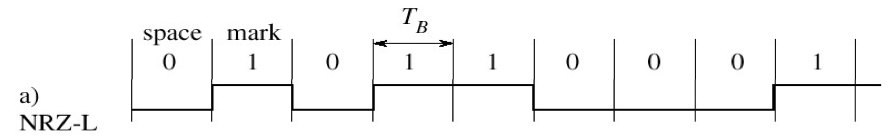
\includegraphics[width=\textwidth]{images/nrz.png}
  \caption{Non-Return-Zero}
  \label{fig:nrz}
  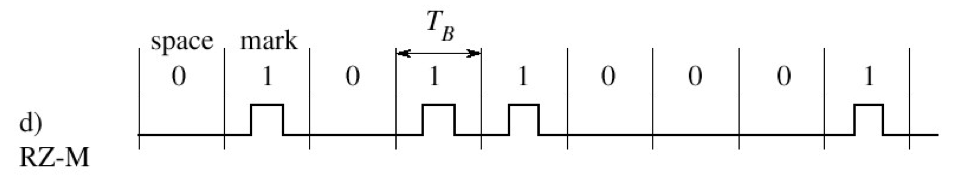
\includegraphics[width=\textwidth]{images/rz.png}
  \caption{Return-Zero}
  \label{fig:rz}
  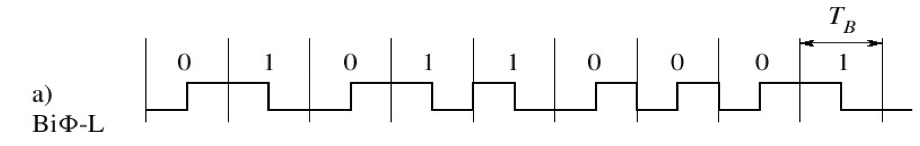
\includegraphics[width=\textwidth]{images/manch.png}
  \caption{Manchester Encoding}
  \label{fig:manch}
  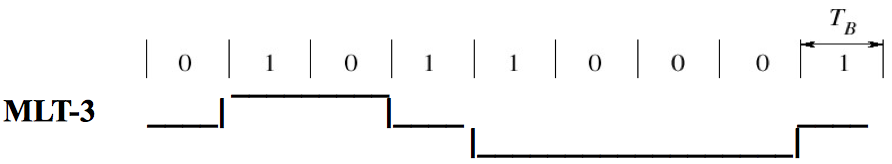
\includegraphics[width=\textwidth]{images/mlt.png}
  \caption{MultiLevel}
  \label{fig:mlt}
\end{figure}

% PARTE C7 - ELAPMISC7
\subsection{Parte C7}\label{c7}
L'integrità del segnale è fondamentale che venga mantenuta al fine di una corretta comprensione tra driver.\\
I disturbi più comuni sono:
\begin{itemize}
  \item \textbf{Crosstalk}: Passaggio di segnale tra due ``canali''.
  \item \textbf{Tra conduttori diversi}: Accoppiamenti induttivi o capacitivi.
  \item \textbf{Su stesso conduttore}: GND $\rightarrow$ Segnali + Alimentazione.
  \item \textbf{Dominio tempo}: Interferenza simbolica.
\end{itemize}
\paragraph{Somma dei crosstalk} Si possono generare due tipi di diafonia, quella \textbf{diretta} dove i disturbi vengono via via generati all'avanzare del gradino con un disturbo di durata costante ma di ampiezza variabile, oppure quella \textbf{inversa} dove i disturbi si affiancano nel tempo, con un disturbo di ampiezza costante ma durata variabile. Sulla linea compare la sempre la somma dei due.
\paragraph{Riduzione crosstalk} Il disturbo è legato principalmente alla velocità dei fronti, agli accoppiamenti ed ai margini di rumore del receiver. Per riddurre questo contributo possiamo quindi rallentare i fronti, ridurre la capacità o le induttanze di accoppiamento o usare segnali differenziali.
\paragraph{Rumore di commutazione} Le correnti di alimentazione relative a parti diverse del circuito possono avere percorsi comuni provocando quindi ground bounce o commutazione simultanea di più uscite.\\
Il nostro obbiettivo di ridurre questi disturbi può essere raggiunto utilizzando condensatori di disaccoppiamento pilotanti carichi a bassa induttanza (in modo da compensare le correnti impulsive) e ricaricati in tempi lunghi.

% Parte D
\section{Parte D}\label{d}
% PARTE D1 - ELAPMISD1
\subsection{Parte D1}\label{d1} % 21 Dicembre 2016
I sistemi di conversione sono ad oggi comunissimi e diffusi ovunque, dal personal computer allo smartphone.
\paragraph{Campionamento} I segnali analogici, essendo reali, sono sempre continui sia in tempo che in ampiezza. La conversione di grandezze fisiche in grandezze numeriche prevede di campionamento (\textit{discretizzazione sui tempi}) e quantizzazione (\textit{discretizzazione sulle ampiezze}).\\
Ad oggi tutti i sistemi elettronici migrano verso il digitale per gli innumerevoli vantaggi legati all'integrità del segnale. Discretizzare un segnale potenzialmente constituisce una perdità di informazioni se non fatto a dovere. Un esempio in figura \ref{fig:delta}.

\begin{figure}[!hp]
  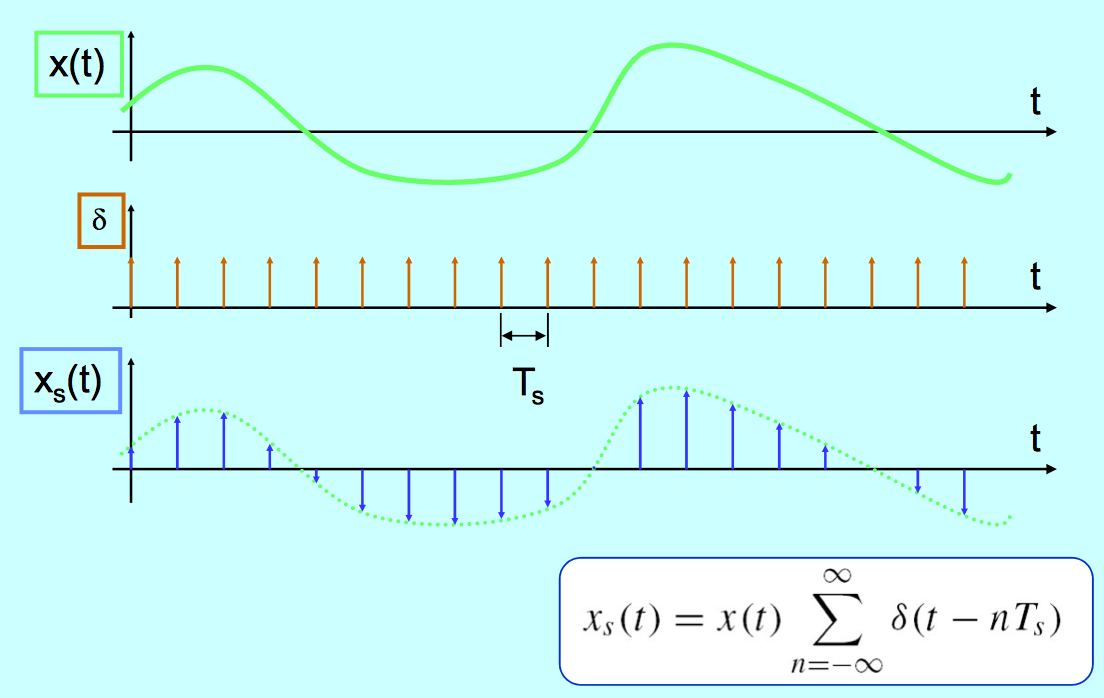
\includegraphics[width=\textwidth]{images/delta.png}
  \caption{Moltiplicazione per un treno di delta per campionare un segnale A}
  \label{fig:delta}
\end{figure}

\paragraph{Campionamento} Un segnale campionato necessità di una ``pulizia'' dagli spettri ripetuti generati dal processo di discretizzazione. Tale processo viene effettuato per mezzo di un filtro passa basso, se però la $F_{S}<2F_{M}$ gli spettri di questo segnale si vanno a sovrapporre generando il fenomeno dell'aliasing con consugente ed irreversibile perdita dei dati.

\paragraph{Filtri anti aliasing} Un possibile soluzione a questo fenomeno è quella di utilizzare un filtro apposito che rispetti le seguenti caratteristiche:
\begin{itemize}
  \item Frequenza di campionamento $F_{S}$ pari almeno al doppio della frequenza del segnale (criterio di Nyquist).
  \item La banda del segnale deve essere limitata.
  \item Rumore di aliasing presente (attenuazione finita).
\end{itemize}

\paragraph{Moduli Sample \& Hold} Il convertitore opera sui singoli campioni e la conversione non è istantanea per tanto durante questa valutazione il segnale va mantenuto stabile.\\
Il modulo S\&H prevede campionamento (\textbf{sample}) e mantenimento (\textbf{hold}) come in figura \ref{fig:seh}.

\begin{figure}[!hpt]
  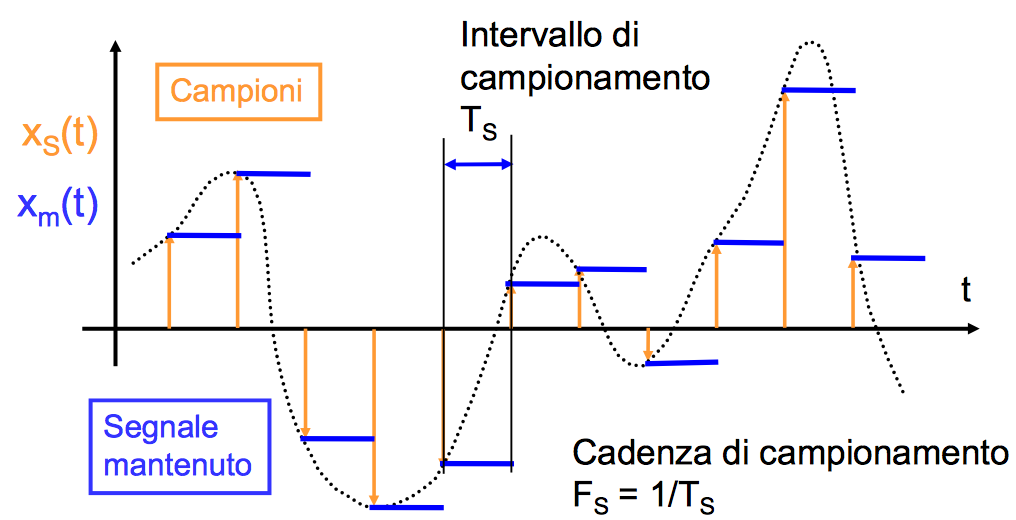
\includegraphics[width=\textwidth]{images/seh.png}
  \caption{Funzionamento modulo Sample \& Hold}
  \label{fig:seh}
\end{figure}

La fase più critica è quella di mantenimento infatti essa trasforma impulsi in gradi di una certa larghezza, moltiplicando quindi lo spettro per $\frac{\sin(F)}{F}$ attenuando quindi le componenti ad elevata frequenza.\\
Processo inverso invece per la ricostruzione del segnale dove sarà necessario tener conto della distorsione spettrale dovuta dalla fase di hold.

\paragraph{Quantizzazione} Questo processo è necessario per definire i valori digitali che verranno generati dalla conversione A/D, il numero di valori è legato dalla relazione $N_{val}=2^{N_{bit}}$. Aumentando il numero di bit di precisione andiamo ad aumentare il numero di possibili valori rappresentabili, il numero di essi non sarà mai infinito quindi si introdurrà un errore di quantizzazione $\epsilon_{q}$ sempre compreso tra tra il massimo discostamento possibile dal valore centrale ovvero $|\epsilon_{q}| \leq \frac{S}{2^{N+1}}$. Non sempre questo valore risulta essere distribuito uniformemente.

\paragraph{SNR} Altro interessante valore è quello del rapporto $SNR_{q}=\frac{Potenza Segnale}{Potenza\epsilon_{q}}$ misurato in $dB$.

\paragraph{Convertitore} La struttura completa di un convertitore A $\rightarrow$ D $\rightarrow$ A si presenta come in figura \ref{fig:ada}.\\
Un parametro interessante di ogni strumento è \textbf{ENOB} \textit{Effective Number Of Bits} rappresenta il numero di bit effettivamente significativi per un convertitore, esso tiene anche conto del valore di $SNR_{tot}$

\begin{figure}[!hpt]
  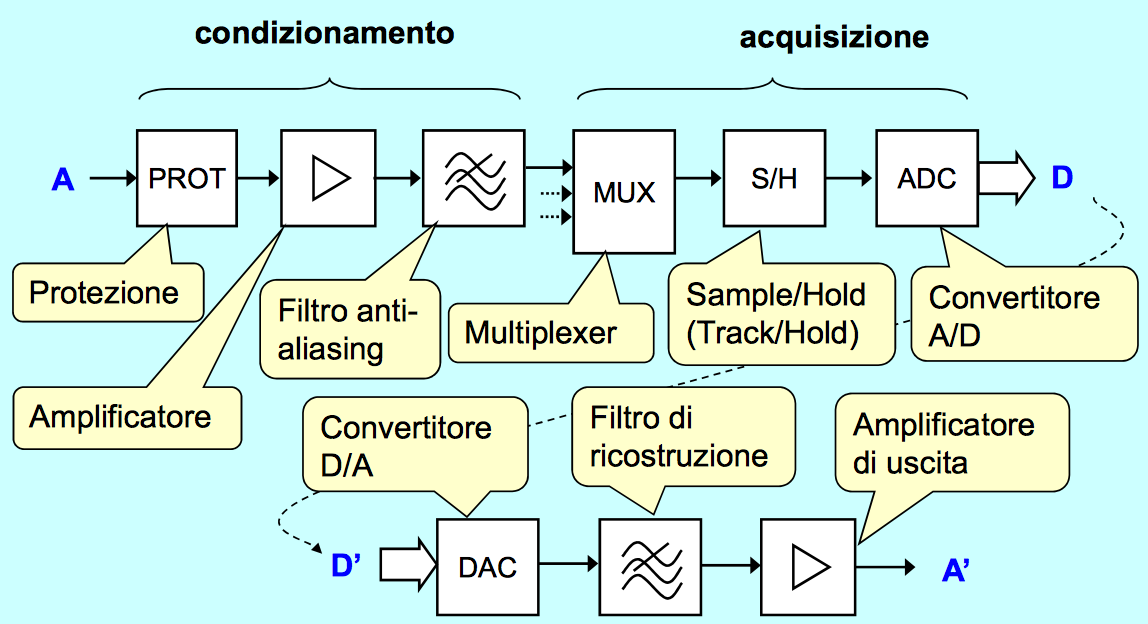
\includegraphics[width=\textwidth]{images/ada.png}
  \caption{Schema convertitore ADA}
  \label{fig:ada}
\end{figure}

% PARTE D2 - ELAPMISD2
\subsection{Parte D2}\label{d2}
I convertitori \textbf{D/A} vengono molto utilizzati, si possono distinguere per una paramentro principale la loro caratteristica di conversione. Maggiore sarà la sequenza dei punti migliore sarà la conversione, quasi a tendere ad una linea continua.
\paragraph{Errori} Gli errori introdotti da un sistema di conversione D/A sono principalmente di due tipi:
\begin{itemize}
  \item \textbf{Statici}: Segnale costante e comportamento a regime.
  \item \textbf{Dinamici}: Segnale ingresso variabile e comportamento in transitorio.
\end{itemize} % 28 Dicembre 2016

\paragraph{Errori Statici} Idealmente la caratteristica del convertitore ideale è una retta, nella realtà non è così, dobbiamo quindi approssimarla nel migliore dei modi.\\
Chiaramente l'introduzione di un approssimazione porta ad una generazione di errori, \textit{non linearità} e \textit{offset}. Vedi figura \ref{fig:caratt}.

\begin{figure}[!hpt]
  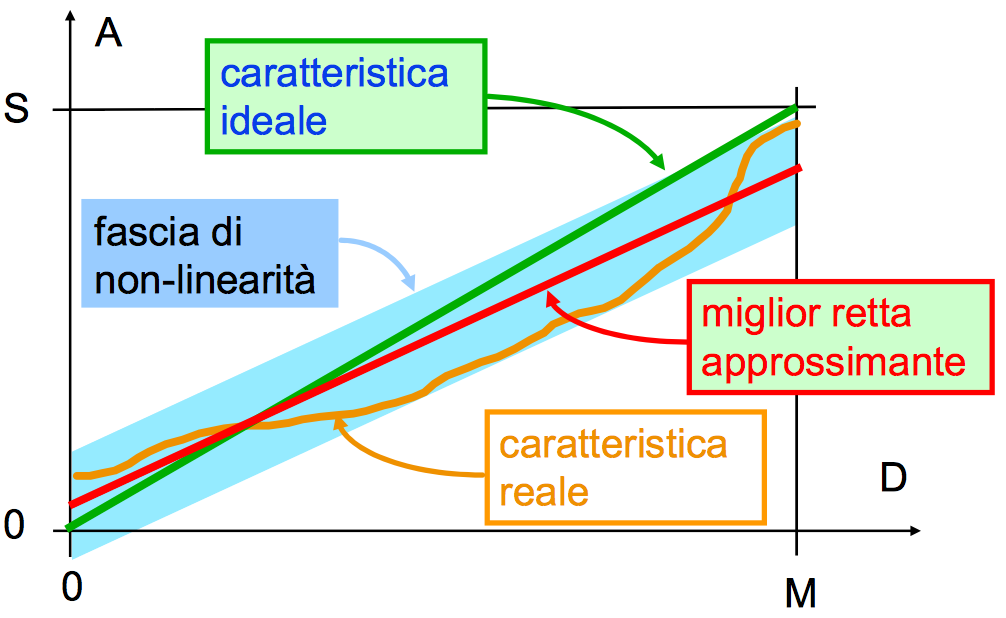
\includegraphics[width=\textwidth]{images/caratt.png}
  \caption{Caratteristica di A/D}
  \label{fig:caratt}
\end{figure}

\paragraph{Errori Lineari}
Uno dei principali errori si genera quando la retta aprossimante non passa per il punto di inizio e fine, tale errore è possibile correggerlo con due parametri. Gli errori da considerare sono:
\begin{itemize}
  \item \textbf{Offset}: Discostamento dalla retta approssimante dal valore 0.
  \item \textbf{Guadagno}: Differenza di pendenza tra la retta originale e quella approssimante.
\end{itemize}

\paragraph{Errori non lineari} Questi errori sono generati nel cofrontare la transcaratteristica reale e retta approssimante. Vengono definiti due tipi di non linearità quella integrale (complessiva) e quella differenziale (locale).\\
La prima valuta il valore complessivo di discostamento, mentre la seconda va ad esaminare un piccolo tratto della caratteristica di conversione.

\paragraph{Errori Dinamici} Esistono due tipologie, il \textit{tempo di assetto} ($T_{S}$) che corrisponde al tempo necessario, all'uscita, a stabilizzarsi sul nuovo valore e il \textit{glitch} ovvero brevi momenti in cui l'uscita può presentare valori molto differenti rispetto al valore iniziale o finale, questo fenomeno è generato dalle differenze nei ritardi di commutazione.

\paragraph{Circuiti per convertitori} Vi sono molteplici soluzioni per generare un convertitore D/A. Ambe due i tipi di conversione possono essere gestiti con uscita in corrente o tensione.\\
La conversione a \textit{grandezze uniformi} somma variabili di ugual peso inserite in quantità corrispondente al valore dell'ingresso digitale.\\
La conversione a \textit{grandezze pesate} somma variabili di peso corrispondente alle potenze di 2, inserito o meno a seconda del valore del bit corrispondente. Per ottenere questo soluzioni si usano resistenze con valore correlati dalla relazione $R2^{N-1}$ per questo la dinamica di uscita potrebbe essere problematica. Una possibile soluzione può essere quella di utilizzare una rete a scala. I vantaggio sono:

\begin{itemize}
  \item Espansione a piacare.
  \item Resistenze solo di valore R o 2R.
  \item Conversione Norton/Thevenin per ottenere uscite in tensione.
\end{itemize}

\paragraph{Errori con grandezze pesate} L'errore sull'uscita dipende dal $pesoramo*erroreramo$ e contribuisce solamente quando esso vale 1, il valore del peso parte dal S/2 fino e si dimezza via via.

% PARTE D3 - ELAPMISD3
\subsection{Parte D3}\label{d3}
Anche nel caso di convertitori \textbf{A/D} vi sono errori analoghi.\\
I tipi di convertitore variano in base a \textbf{velocità} e \textbf{complessità} direttamente proporzionali tra loro e sfruttano una struttura di comparatori e logica come in figura \ref{fig:ad_gen}.

\begin{figure}[!hpt]
  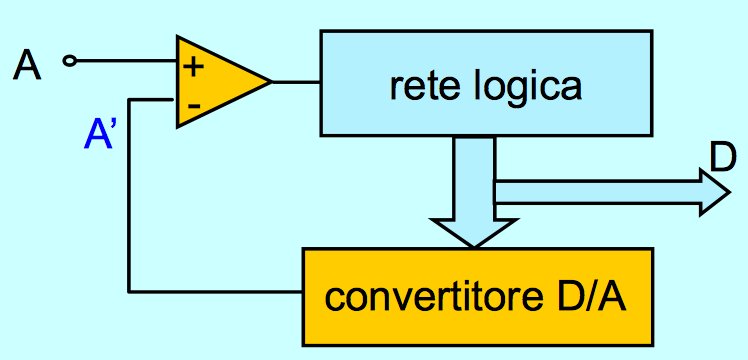
\includegraphics[width=\textwidth]{images/ad_gen.png}
  \caption{A/D Generico}
  \label{fig:ad_gen}
\end{figure}

\paragraph{Convertitori Flash} Questo tipo di convertitori sfrutta $2^N-1$ comparatori di soglia, viene spesso chiamato convertitore in parallelo per via della conversione di N bit in un singolo ciclo di clock. E' di complessa realizzazione e veloce, molto utilizzato nella conversione di segnali a larga banda.
\paragraph{D/A in reazione} La base di questo circuito è quello di utilizzare una rete logica in grado di variare D fino a che approssimi il meglio possibile il valore di ingresso. Le soluzioni possibili sono quella ad inseguimento o ad approssimazioni successive.
\paragraph{Convertitore ad inseguimento} Il funzionamento è molto semplice viene confrontato il segnale di ingresso (A) con quello generato dalla rete logica (A') se $A'<A$ il contatore viene incrementato e decrementato nel caso opposto. Nel caso di un segnale costante il valore continuerà a generare una gradinata attorno al valore originale. Il problema potrebbe manifestarsi nel caso di variazioni del segnale troppo veloci. Si tratta di un componente semplice (1 comparatore) ma lento ($2^N$ cicli $\rightarrow$ N bit).
\paragraph{Conv. approssimazioni successive} Il segnale di ingresso viene confrontato son S/2 determinando MSB da cui deriverà il confronto successivo che andrà a determinare MSB -1 e così via.\\
Il componente è abbastanza semplice (1 comparatore) e discretamente veloce (N cicli $\rightarrow$ N bit), è più lento rispetto al convertitore flash ma più veloce rispetto a quello ad inseguimento. Vedi figura \ref{fig:ap_succ}

\begin{figure}[!hpt]
  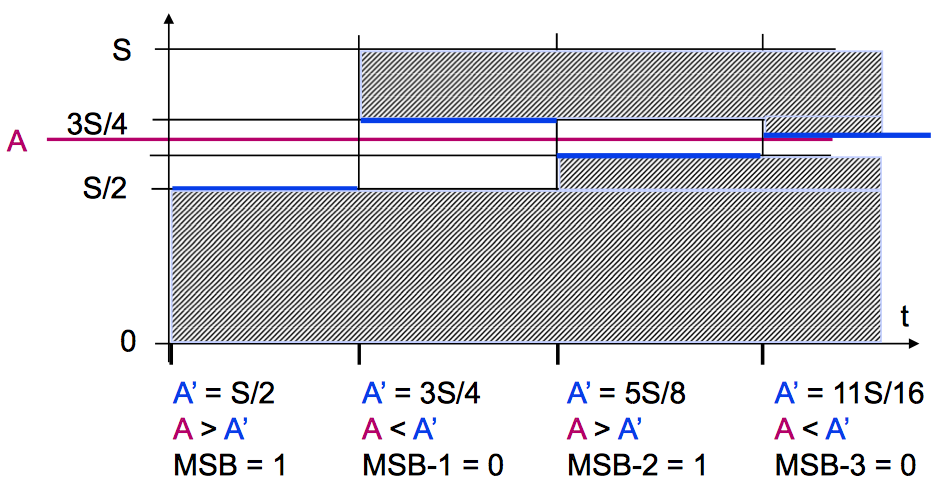
\includegraphics[width=\textwidth]{images/ap_succ.png}
  \caption{Approssimazione successiva}
  \label{fig:ap_succ}
\end{figure}

% PARTE D4 - ELAPMISD4
\subsection{Parte D4}\label{d4}
In questa sezione verranno trattate altre possibili strutture per convertitori A/D.
\paragraph{Conversione a residui} Questo tipo di convertitore si basa su quello visto precedentemente (cap. \ref{d3}) ad approssimazioni successive. La differenza riguarda la logica e la maggiore complessità. Utile nell'utilizzo con la tecnica a pipeline. Il quale permette di ottenere, con l'aggiunta di moduli S/H, gli stessi tempi di conversione con però solo N comparatori con i $2^N$ del flash.\\
In figura \ref{fig:adconfr} possiamo vedere un rapido riepilogo delle tecniche descritte.

\begin{figure}[!hpt]
  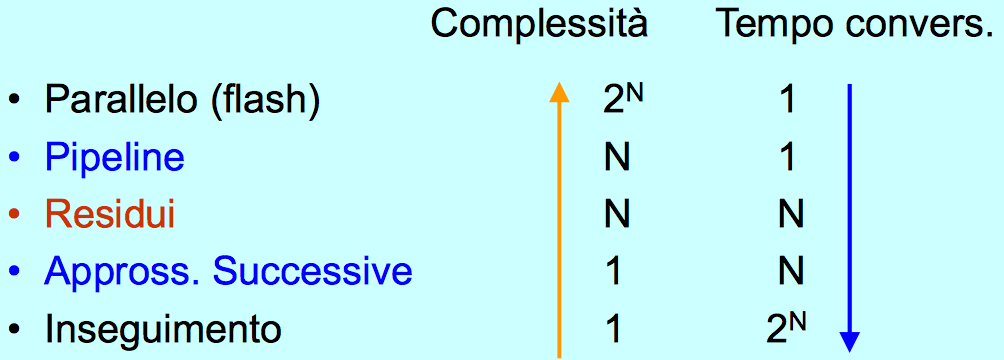
\includegraphics[width=\textwidth]{images/adconfr.png}
  \caption{Confronto tra strutture di conversione A/D}
  \label{fig:adconfr}
\end{figure}

\paragraph{Conversione differenziale e delta} %1 Gennaio 2017
Il convertitore differenziale fornisce un flusso seriale di bit ad alta cadenza corrispondenti al comando UP/DOWN sul comparatore di soglia nel A/D ad inseguimento.\\
Nel convertitore $\Delta$ vengono generate una serie di impulsi a cadenza $T_{clk}$ ricostruiti successivamente da un integratore. Alcune considerazioni in merito al convertitore $\Delta$:
\begin{itemize}
  \item Non richiede componenti precisi.
  \item Dinamica limitata.
  \item Presenta livelli minimi e massimi.
  \item Dinamica per $T_{clk}$: $\frac{\gamma}{2}<V<\frac{\gamma}{\omega T_{clk}}$
\end{itemize}
Esiste anche il convertitore $\sigma \Delta$ il quale aggiunge alcune componenti per permetere di convertire segnali a più alta frequenza.

\paragraph{Quantizzazione} Esistono due tipi di quantizzazione, quella lineare e quella logaritmica.\\
Quella \textit{lineare} presenta intervalli di quantizzazione costanti, mentre quella \textit{logaritmica} genera intervalli direttamente proporzionali all'ampiezza del segnale.
Il vantaggio della seconda soluzione è legato all'independenza di SNRq dal livello del segnale.

% PARTE D5 - ELAPMISD5
\subsection{Parte D5}\label{d5}
In questo capitolo verranno analizzate le strutture di multiplexer e moduli sample-hold.

\paragraph{Multiplexer} Il MPX è un sistema a più canali in grado di selezionarne solo 1 tra gli N canali disponibili, chiaramente nello svolgimento di questo compito i segnali non devono essere alterati in alcun modo.\\
La realizzazione più semplice di questa struttura è quella di utilizzare un banco di interruttori con trasistor MOS. Questa tecnica porta alla generazione di alcuni errori non trascurabili:
\begin{itemize}
  \item \textbf{$R_{ON}$}: L'interruttore chiuso ha una resistenza equivalente $R_{ON}$  che andrà a generare un partitore di tensione tra l'ingresso e l'uscita.
  \item \textbf{$I_{OFF}$}: Ogni interruttore aperto ha una corrente di perdita $I_{OFF}$ le quali andranno a generare una tensione di offset in uscita.
  \item \textbf{Limitazione di banda}: Capacità parassite del MPX e del carico limitano la banda del segnale trasferito (generano una cella passa-basso).
\end{itemize}

\paragraph{Sample-Hold} Il comportamento ideale di questo modulo prevede il campionamento di un segnale analogico ed il mantenimento di tale valore per tutta la durata della conversione. Nella realtà il comportamento è leggermente diverso, come in figura \ref{fig:tsh}:
\begin{enumerate}
  \item \textcolor{RedOrange}{\textbf{Acquisizione ed inseguimento (tracking)}}.
  \item \textcolor{Red}{Campionamento (sampling)}.
  \item \textcolor{Green}{Mantenimento (hold)}.
\end{enumerate}

\begin{figure}[!hpt]
  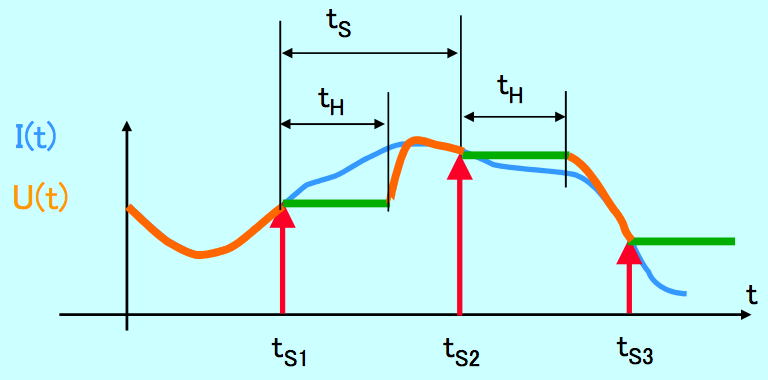
\includegraphics[width=\textwidth]{images/tsh.png}
  \caption{Track - Sample - Hold}
  \label{fig:tsh}
\end{figure}

Il circuito risulta realizzabile come riportato in figura \ref{fig:th}, con SW chiuso avremo la fase di TRACK mentre SW aperto saremo in HOLD.

\begin{figure}[!hpt]
  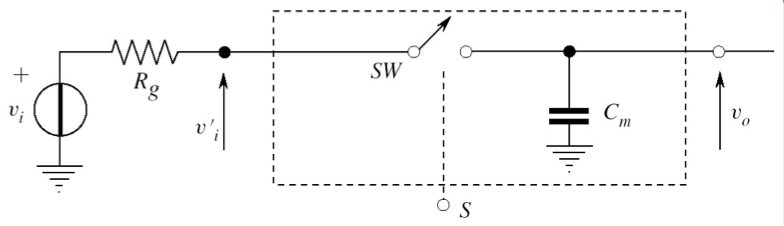
\includegraphics[width=\textwidth]{images/th.png}
  \caption{Circuito Track/Hold}
  \label{fig:th}
\end{figure}

Il campionamento non è esente da errori, oltre a quelli riportati nel capitolo \ref{d1}, vengono introdotti ulteriori errori legati al modulo S/H dovuti principalmente al ritardo di apertura dei SW. Anche la fase di mantenimento genera problemi infatti la carica sul condensatore varia (\textit{errore di decadimento}, scarica su $R_{L}$), l'imperfetto isolamento del segnale (\textit{errore di feedthrough}, passaggio di cariche con SW aperto) o la polarizzazione del dielettrico.

% PARTE D6 - ELAPMISD6
\subsection{Parte D6}\label{d6}
Questa sezione tratterà le rimanenti parti nei circuiti di acquisizione come protezione, amplificatori, ecc...
\paragraph{Circuiti di protezione} I CP sono parti necessarie dei moduli di acquisizione progettati in modo da proteggere il circuito dal danneggiamento, alcune soluzioni sono:
\begin{itemize}
  \item Clamp a diodi (\textit{$V_{OUT}$ limitata tra $V_{al}+$ e $V_{al}-$.})
\end{itemize}

\paragraph{Condizionamento} I convertitori possono avere molteplici ingressi per questo necessiteremo di \textbf{amplificatore di condizionamento} in modo da adattare il segnale come dinamica e come tipo. Vi sono molteplici tipologie:
\begin{itemize}
  \item Amplificatori V/V o I/I o convertitori V$\rightarrow$I o I$\rightarrow$V.
  \item Ingresso single-ended o differenziale.
  \item Uscita single-ended o differenziale.
\end{itemize}

Le ultime due tipologie devono rispettare alcune caratteristiche ovvero \textbf{amplificare} (di un valore noto) i segnali differenziali $A_{D}$ e \textbf{non amplificare} (attenuare) i segnali di modo comune $A_{C}$, dove il rapporto $A_{D}$/$A_{C}$ prende il nome di CMRR (Common Mode Rejection Ratio).

\paragraph{Filtri} Come analizzato rapidamente nel capitolo \ref{d1} è necessario ``pulire'' il nostro segnale dagli spettri prodotti dal campionamento. Per fare ciò è necessario un filtro (aliasing), nel nostro caso uno di tipo passa-basso.\\
I filtri possono ottenere solo approssimazione del segnale ideale. Le tecniche di realizzazione di questo componente sono principalmente due:
\begin{itemize}
  \item \textbf{Analogica}:
  \begin{itemize}
    \item Passivi: LC
    \item Attivi: Amp. Op. + RC
    \item Capacità commutate (attualmente molto usata)
  \end{itemize}
  \item \textbf{Digitale}: Richiedono conversione A/D e D/A e portano con se tutti i vari errori del caso (vedi capitoli \ref{d2}-\ref{d4}). Realizzabili tramite FF, porte, FPGA, ecc...
\end{itemize}

Tra le varie fasi di progetto di questi filtri vi è quella della scelta del tipo di approssimazione, ne illustriamo brevemente tre:
\begin{itemize}
  \item \textbf{Bessel}: Fase lineare, ritardo di gruppo costante, nessuna distorsione e nessuna ondulazione in banda passante.
  \item \textbf{Butterworth}: Ritardo di gruppo variabile (distorsione) e nessuna ondulazione in banda passante.
  \item \textbf{Chebicheff}: Ondulazione in banda passante e forte attenuazione fuori banda.
\end{itemize}

% Parte E
\section{Parte E}\label{E}
Sezione riguardante i circuiti di potenza e relative componenti.
% PARTE E1 - ELAPMISE1
\subsection{Parte E1}\label{e1} %3 gennaio 2017
La gestione della potenza è un discorso molto importante, il compito viene principalmente demandato all'alimentatore il quale dovrà fornire energia ai vari moduli partendo da diverse sorgenti, gestendo una tensione in uscita ben definita al variare dell'ingresso.

\paragraph{Diodi Zener} Ogni giunzione ha una propria tensione di breakdown (o rottura) oltre la quale vi sono possibili danni, talvolta permanenti, ai circuiti. Alcuni dispositivi lavorano in quella zona come il diodo Zener spesso usato come circuito di protezione o regolatore di tensione. Il diodo in questione è basato sulla polarizzazione inversa.

\paragraph{BJT e MOS-FET di potenza} Questi due componenti vengono spesso usati anche in circuiti di potenza, per semplicità verranno analizzate le differenze tra i due.
\begin{itemize}
  \item MOS-FET usa portatori maggioritari.
  \begin{itemize}
    \item Elevatà capacità di commutazione.
    \item Ridotta dipendenza dalla temperatura.
  \end{itemize}
  \item MOS-FET richiede circuiti di pilotaggio più semplici.
  \item STATO ON:
  \begin{itemize}
    \item BJT: $V_{CEsat} + R_{ON}$
    \item MOS: $R_{ON}$
  \end{itemize}
  \item STATO OFF: Correnti di perdita (leakage)
\end{itemize}

\paragraph{SOA} La \textit{Safe Operating Area} è costituita da tutte quelle regole che permettono un corretto utilizzo del componente descritto. I limiti operativi classici sono:
\begin{itemize}
  \item Tensione di Breakdown
  \item Corrente massima
  \item Potenza massima
  \item Temperatura massima
  \item Applicazioni speciale (resistenza alle radiazioni, vibrazioni, ecc...)
\end{itemize}

\paragraph{Potenza dissipata} Ogni dispositivo sissima una potenza ($P_{diss} = V I$), questo parametro determina l'aumento di temperatura, un valore NON trascurabile. Il calore generato dovrà essere gestito e dissiapato in modo da consentire un corretto lavoro da parte dei componenti.\\
Altra considerazione in merito alla potenza è la sua non costanza infatti essa è inversamente proporzionale alla temperatura.

\paragraph{Dissipazione in BJT e MOS} Nel caso di condizioni ON o OFF la potenza è pressochè nulla, gli stadi intermedi invece sono gli unici ad avere dissipazione.

% PARTE E2 - ELAPMISE2
\subsection{Parte E2}\label{e2} %3 gennaio 2017
I sistemi di alimentazione possono essere molteplici, AC, DC, batterie, ecc... Per questo motivo dovremo spesso convertire la nostra fonte in modo da poterla utilizzare. Durante questa conversione chiaramente dobbiamo avere le minime perdite, parametri ben controllabili e sicurezza. Ecco alcuni possibili parametri:
\begin{itemize}
  \item Ingresso:
  \begin{itemize}
    \item Tipo: AC, DC, batteria, dinamo, ecc...
    \item Valore e campo: 100-240V AC, 12V DC $\pm$ 10\%
    \item Frequenza: 50 Hz
    \item Rumore e spurie: Armoniche, transitori, ecc...
  \end{itemize}
  \item Uscita:
  \begin{itemize}
    \item Valori nominali: Tensione, corrente, ondulazione e rumore
    \item Stabilità: Relazione al variare del carico
    \item Altro: Foldback, fail safe, protezioni, temperatura, ecc...
  \end{itemize}
\end{itemize}

Lo schema a blocchi di PSU (\textit{Power Supply Unit}) in figura \ref{fig:psu} da cui verranno analizzati tutti i blocchi.

\begin{figure}[!hpt]
  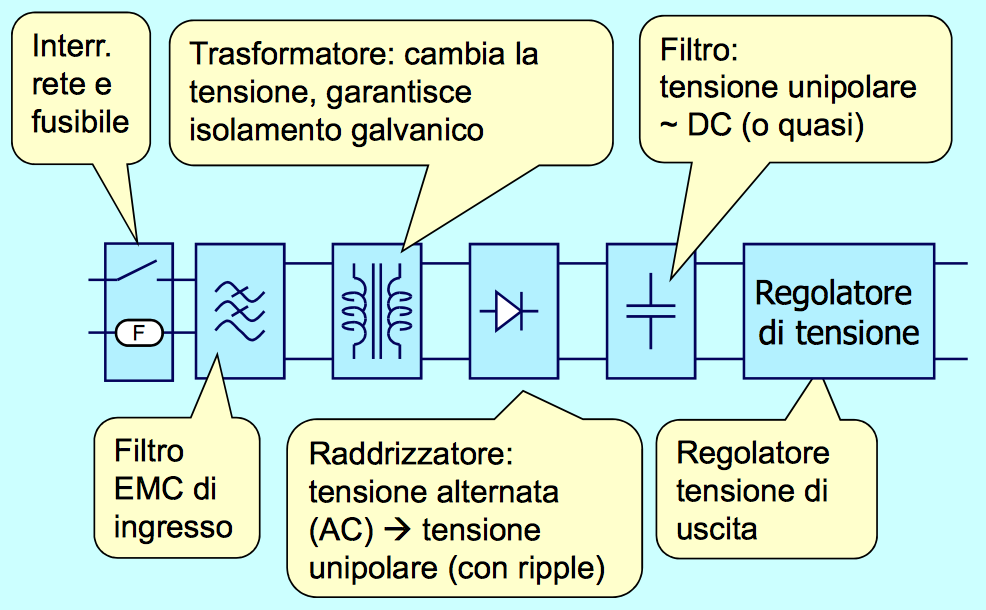
\includegraphics[width=\textwidth]{images/psu.png}
  \caption{Schema a blocchi PSU}
  \label{fig:psu}
\end{figure}

\paragraph{Maglie di ingresso} L'interruttore ON/OFF di rete serve ad isolare l'alimentazione, non è sempre presente. Il filtro (passivo) blocca le interferenze condotte mentr il fusibile apre per correnti eccessive per protezione. Il trasformatore porta la tensione ad un valore ``comodo'' e garantisce isolamento galvanico, ad oggi spesso sostituito da alimentatori a commutazione.

\paragraph{Conversione AC-DC} Questa trasformazione necessità di due elementi base, il raddrizzatore ed il filtro anti-ronzio.\\
Il raddrizzatore di occupa di trasformare AC da bipoare ad unipolare usando diodi, la tensione raddrizzata ha una componente DC e numerose componenti AC (aromiche di rete).
Il filtro anti-ronzio invece ha il compito di far transitare la componente DC senza attenuazione e pulendola dalle componenti AC tramite circuiti passivi (RC, LC) o attivi (regolatore di tensione).\\

\paragraph{Raddrizzatori} Vi sono più tipologie di raddrizzatori a \textbf{singola semionda} (vedi figura \ref{fig:semi}) o ad \textbf{onda intera} (vedi figura \ref{fig:intera}).

\begin{figure}[!hbpt]
  \centering
  \begin{minipage}{.45\textwidth}
    \centering
    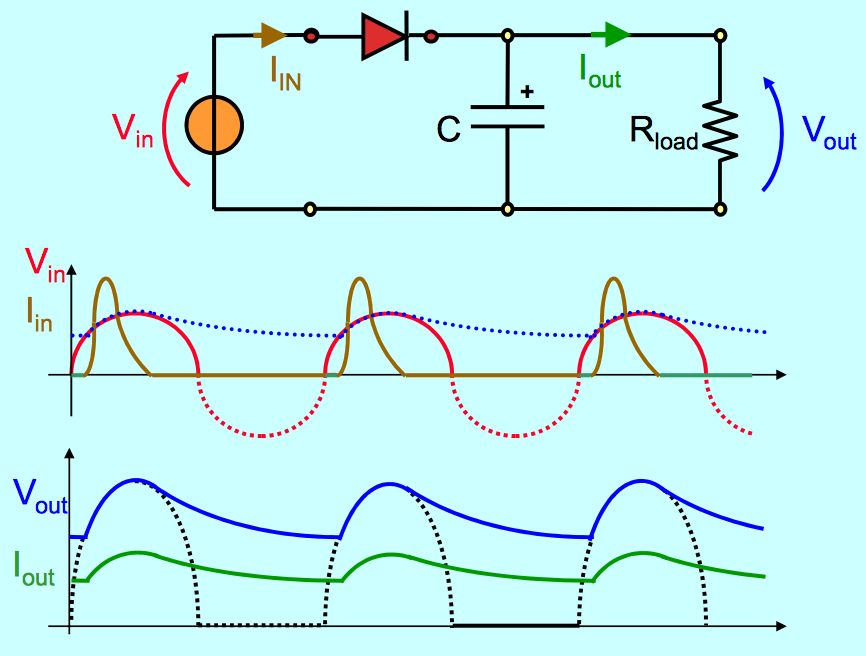
\includegraphics[width=\linewidth]{images/semi.png}
    \caption{Raddrizzatore a semi-onda}
    \label{fig:semi}
  \end{minipage}\hfill
  \begin{minipage}{.45\textwidth}
    \centering
    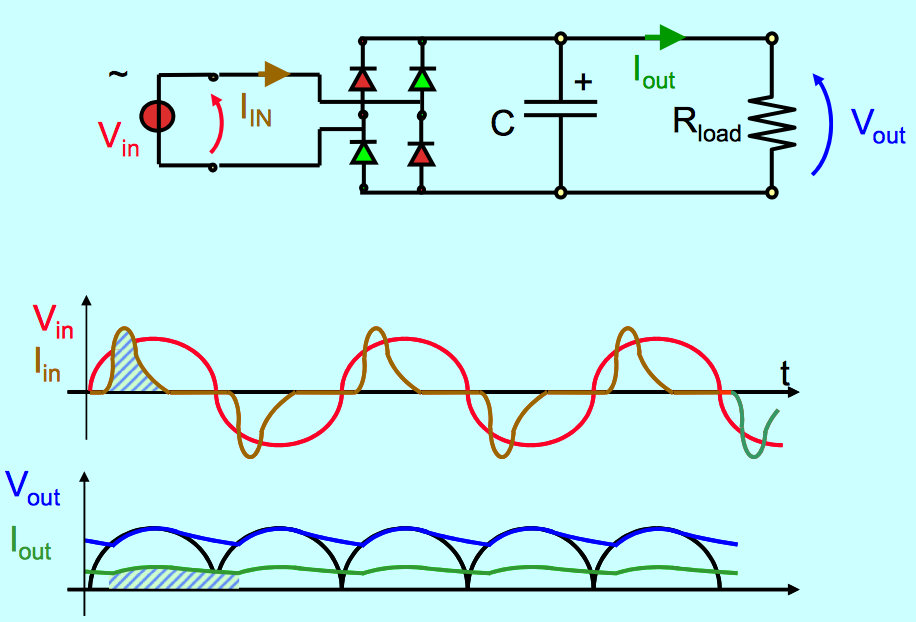
\includegraphics[width=\linewidth]{images/intera.png}
    \caption{Raddrizzatore a onda intera}
    \label{fig:intera}
  \end{minipage}\hfill
\end{figure}

Il flusso della corrente non è costante, nel primo ciclo il condensatore di filtro si caricherà completamente (corrente inrush), mentre a regime la corrente di picco sarà molto più alta della corrente media con conseguente ondulazione all'uscita. Per poter migliorare i parametri ondulatori sarebbero necessari filtri con alte capacità o forti correnti impulsive oppure utilizzare strutture alternative come alimentatori a commutazione.

\paragraph{Regolatore di tensione} Questo componente ha il compito di fornire una tensione di uscita $V_{O}$ costante per valori variabili di $V_{i}$ e L.\\
Nel caso del regolatore parallelo si andrà a creare un partitore di corrente dove, agendo sul ramo parallelo, si andrà a variare il rapporto di partizione. Realizzabile, molto semplicemente e con bassa efficenza, con diodi Zener.\\
In quello serie invece si modificherà il rapport agendo sul ramo serie. Questo tipo di circuito si comporta come una resistenza variabile controllata (implementabile con BJT o MOS, Amplificatori, ecc...).

% PARTE E3 - ELAPMISE3
\subsection{Parte E3}\label{e3} % 3 gennaio 2017 - 19:18
Il compito dei regolatori a commutazione è quello di permettere, come uno SW, di controllare la potenza erogata.
\begin{itemize}
  \item \textbf{ON}$\rightarrow$Piena Potenza (con filtro)
  \item \textbf{OFF}$\rightarrow$Potenza Zero
\end{itemize}
Idealmente dovrebbe essere fatto senza perdite ma non è possibile. L'energia filtrata dal passa-basso viene fornita al carico come onda rettangolare, con valor medio legato al duty cycle. Il filtro può essere di due tipi, RC (perdite nella R, basse potenze) o LC (basse perdite, potenze elevate).\\
Vi sono diverse possibilità nella scelta della topologia dei regolatori. Il vantaggio è il loro alto rendimento, l'uniche note negative sono invece la generazione di ondulazioni ed interferenze.

\paragraph{Buck} Questo regolatore presenta due interruttori complementari, nel caso di SW1=ON la lorrente in L (induttore) cresce e viceversa con SW2=ON. Spesso SW2 viene realizzato con un diodo che, polarizzato inversamente, regolerà correttamente il flusso. In generale $V_{OUT}<V_{IN}$. (Figura \ref{fig:buck})

\paragraph{Boost} Molto simile al buck, ma scambia SW1 con l'induttanza mentre SW2 viene realizzato con un diodo. In generale $V_{OUT}>V_{IN}$. (Figura \ref{fig:boost})

\paragraph{Buck-Boost} Combina le due tipologie precedentemente descritte generando una tensione di polarità invertita. (Figura \ref{fig:buckboost})

\paragraph{Fly-Back} La caratteristica principale è l'isolamento galvanico, si presenta come un regolatore buck-boot con un trasformatore al posto dell'induttanza. Per la regolazione invece occorre una reazione isolata. (Figura \ref{fig:flyback})

\begin{figure}[!hbpt]
  \centering
  \begin{minipage}{.45\textwidth}
    \centering
    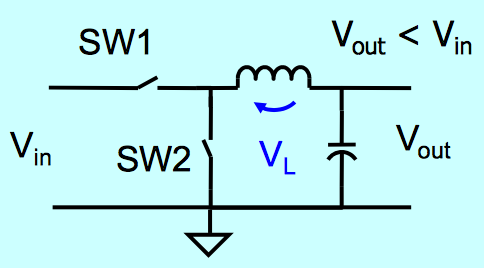
\includegraphics[width=\linewidth]{images/buck.png}
    \caption{Regolatore Buck}
    \label{fig:buck}
  \end{minipage}\hfill
  \begin{minipage}{.45\textwidth}
    \centering
    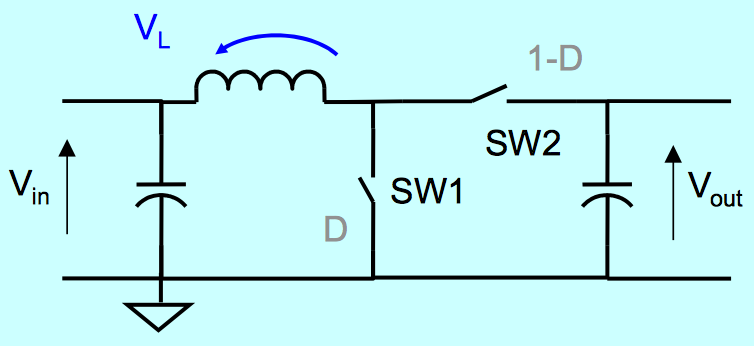
\includegraphics[width=\linewidth]{images/boost.png}
    \caption{Regolatore Boost}
    \label{fig:boost}
  \end{minipage}\hfill
\end{figure}

\begin{figure}[!hbpt]
  \centering
  \begin{minipage}{.45\textwidth}
    \centering
    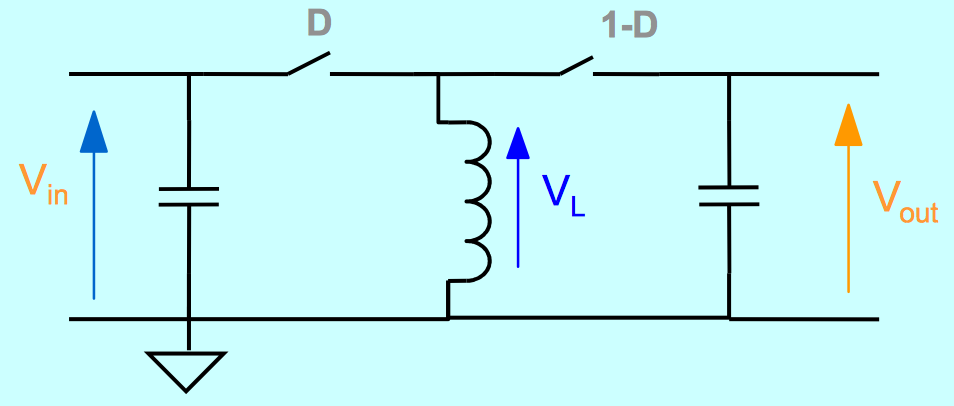
\includegraphics[width=\linewidth]{images/buckboost.png}
    \caption{Regolatore Buck-Boost}
    \label{fig:buckboost}
  \end{minipage}\hfill
  \begin{minipage}{.45\textwidth}
    \centering
    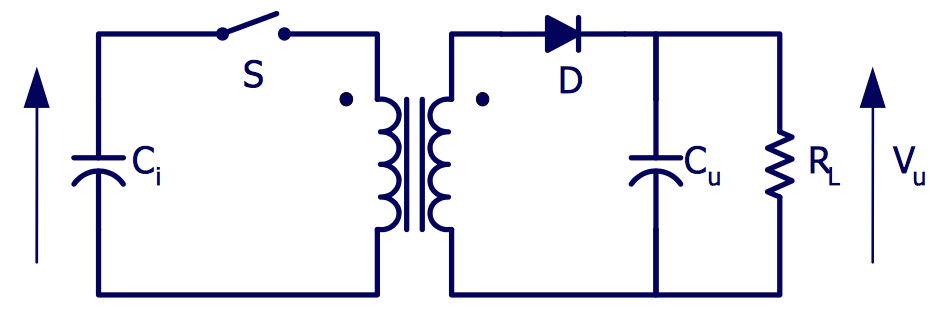
\includegraphics[width=\linewidth]{images/flyback.png}
    \caption{Regolatore Fly-Back}
    \label{fig:flyback}
  \end{minipage}\hfill
\end{figure}

% PARTE E4 - ELAPMISE4
\subsection{Parte E4}\label{e4} % 4 gennaio 2017 - 10:57
Le techniche di alimentazione di un circuito sono molteplici, batterie, accumulatori, celle solari, ecc... Andiamo ora ad analizzare alcune sorgenti DC.
\paragraph{Batterie} Le principali caratteristiche di una batterie sono:
\begin{itemize}
  \item Struttura chimico/fisica
  \item Tensione della singola cella
  \item Corrente erogabile: curva di scarica V(I,t)
  \item Durata
  \item Capacità per unità di peso/volume
  \item Modalità e parametri di ricarica (per ricaricabili)
\end{itemize}
Nel caso di batterie \textbf{non ricaricabili} (\textit{primarie}) i parametri chiave saranno $\frac{Wh}{kg}$ e la tensione, citiamo (valori classici):

\begin{center}
\begin{tabular}{ |c|c|c| }
 \hline
 Piombo [Pb] & Nickel [Ni] & Litio [Li] \\
 \hline
 \hline
 2V & 1.2V & 3V \\
 \hline
\end{tabular}
\end{center}

Per quanto riguarda invece le batterie \textbf{ricaricabili} (\textit{secondarie o accumulatori}) un'altro importante parametro da conoscere è il numero di cicli carica/scarica effettuabili. Ne conosciamo diverse tipologie:
\begin{itemize}
  \item \textbf{Piombo [Pb]}: (Lead Acid)
  \begin{itemize}
    \item Grandi capacità basso costo (automobili)
    \item Gruppi continuità (UPS)
  \end{itemize}
  \item \textbf{Nickel - Metal Hydride [Ni-MH]}:
  \begin{itemize}
    \item Media densità di energia
    \item Variante Ni-Cd (Nickel-Cadmio)
  \end{itemize}
  \item \textbf{Lithium Ion [Li-Ion]}
  \begin{itemize}
    \item Doppia densità rispetto alle Ni-xx
    \item Molto diffuse su apparati portatili
    \item In espansione
    \item Costo alto
  \end{itemize}
\end{itemize}

Le modalità di ricarica di una Ni-MH prevedono una carica costante da 1c a 2c ed un mantenimento a batteria carica da c/10 a c/40. Nella batterie Li-Ion la ricarica viene effettuata ad una tensione costante di circa 4.2V con una corrente di 1c (generalmente c/5).

% Parte F
\section{Parte F}\label{F}
Sezione riguardante i voltmetri e le misure in frequenza.
% PARTE F1 - f1-voltmetridigitali
\subsection{Parte F1}\label{f1} % 4 gennaio 2017
Il voltmetro digitale da informazioni sulla tensione sotto forma di numero invece che su scala ad indice. I \textbf{vantaggi} di una soluzione digital sono:
\begin{itemize}
  \item Elimina incertezza di lettura
  \item Facilità di lettura
  \item Resistenza ad urti e vibrazioni
  \item Tempo di risposta piccolo
  \item Potenzialmente poca incertezza
\end{itemize}
I \textbf{difetti} invece possono essere:
\begin{itemize}
  \item Falso senso di precisione
  \item Difficile valutazione di evoluzione (no lancetta in movimento)
  \item Lettura a colpo d'occhio più difficile
\end{itemize}

L'utilizzo di questi strumenti è possibile grazie alla conversione A/D tratta con precisione nei capitoli \ref{d3} e \ref{d4}. Alcune informazioni aggiuntive riguardo al convertitore subranging costituito da una serie di convertitori flash.\\
Da considerare invece con più precisione i convertitori ad integrazione. Nel caso di quelli a singola rampa viene fornita un'uscita legata al valor medio dell'ingresso in un certo intervallo di tempo, questa operazione permette una pulizia degli alias agendo dal filtro passa-basso. Il tempo di integrazione è seglibile dall'operatore, un valore interessante è $T=20 ms$ per eliminare tutti i derivati dalla frequenza di rete a 50Hz e multipli.\\
I convertitori a doppia rampa invece sfruttano la maggior precisione nel calcolare dei tempi valutando la carica e scarica di un ben noto condensatore. Ulteriore evoluzione sono i sistemi a multirampa e gli altri visti nei capitoli \ref{d3} e \ref{d4}.

\paragraph{ADC} L'accuratezza dei convertitori viene espressa dai costruttori un pò a loro favore, in condizioni ottimali. In qualsiasi caso ogni converter un'errore di:
\begin{itemize}
  \item \textbf{Quantizzazione}: Metà dell'intervallo di quantizzazione.
  \item \textbf{Non-linearità differenziale}: Scostamento dalla risposta di un convertitore ideale di un singolo gradino.
  \item \textbf{Non-linearità integrale}: Scostamento massimo della caratteristica di un ADC dal valore di uno ideale.
\end{itemize}

% PARTE F2 - f1-misure tempo e frequenza
\subsection{Parte F2}\label{f2} % 4 gennaio 2017
Tempo e frequenza sono, ad oggi, le grandezze fisiche misurabili con maggior precisione (minor incertezza) questo grazie alla grande disponibilità di campioni e agli ottimi ed economici strumenti.\\
A causa della mancanza di sincronismo tra due segnali si ha sempre una incertezza assoluta di quantizzazione pari a $\pm$ 1 (in termini relativi $\pm\frac{1}{n}$), per ridurla è necessario che n sia il massimo possibile, per questo alle basse frequenze l'incertezza inizia ad avere un peso notevole.\\

% PARTE F3 - f1-voltmetri ac
\subsection{Parte F3}\label{f3} % 4 gennaio 2017
Una qualsiasi grandezza tempo variante richiede molte (al limite infinite) misurazioni per essere caratterizzata. Per il motivo appena citato si preferisce fornire altre informazioni a livello globale, come il \textbf{valor efficace}.\\
Questo valore è molto importante perchè indica il \textit{"valore di tensione costante al quale genereremo la stessa quantità di energia, nello stesso tempo del nostro segnale tempo-variante"}, calcolare questo valore non è però facile e vi sono 3 tipi di voltmetri per calcolarlo. Nel caso di segnali sinusoidali si possono sfruttare le semplice formule:\\
\begin{equation}
  \begin{gathered}
    V_{eff}=\frac{V_{p}}{\sqrt{2}}=\frac{\pi V_{m}}{2\sqrt{2}}
    \label{eq:veff}
  \end{gathered}
\end{equation}
Nel caso di segnali \textbf{non} sinusoidali dobbiamo, dall'indicazione del voltmetro a valor medio divide per 1.11 (ricavando il valore corretto) e nel caso del voltmetro di picco moltiplicare per 1.41.

\paragraph{Valor Medio (raddrizzato)} Questo tipo di strumenti è basato su un raddrizzatore in serie ad un voltmetro a valore medio in DC.

\paragraph{di Cresta} Questo tipo di voltmetri sfrutta un condensatore. Una volta raggiunto il valore di picco come carica nel condensatore la tensione scende aprendo così il diodo, mantenendo il valore da misurare nella capacità. Per alte frequenze basta usare un piccolo condensatore in modo che si carichi velocemente, nella basse frequenze invece diventa più problematica la questione per via della prolungata apertura del diodo. Lo svantaggio principale di questi voltmetri è legato all'impossibilità di separare la componente continua. Una soluzione è quella di scambiare condensatore e diodo in modo da filtrare la DC.

\paragraph{Valore Efficace: RMS - TRMS} Questi strumenti forniscono il valore efficace del segnale indipendentemente dalla forma d'onda. Sfruttano la trasformazione elettrotermica (termocoppia). Il funzionamento della termocoppia è direttamente correlato alla completa dissipazione in forma calore dell'energia elettrica, misurando tale valore possiamo risalire al valore efficace.

% Parte G
\section{Parte G}\label{G}
Sezione riguardante i sensori.
% PARTE G1 - g1-sensori
\subsection{Parte G1}\label{g1} % 4 gennaio 2017
Un \textbf{SENSORE} è un dispositivo che riceve un'informazione da un segnale di ingresso, costituito da una grandezza fisica, e la restituisce mediante un segnale d'uscita, costituito da una grandezza fisica diversa.\\
Al segnale in ingresso risulta sempre associata un certa energia che è scambiata tra sensore e sistema misurato con conseguente perturbazione di entrambi.\\
Esistono due tipi di sensori:
\begin{itemize}
  \item \textbf{ATTIVI}: Visti come generatori di tensione, corrente o carica
  \begin{itemize}
    \item Fotoelettrico
    \item Termoelettrico
    \item ecc...
  \end{itemize}
  \item \textbf{PASSIVI}: Visti come impedenze
  \begin{itemize}
    \item Temperatura $\rightarrow$ Resistività
    \item Irraggiamento $\rightarrow$ Resistività
    \item Umidità $\rightarrow$ Capacità
    \item ecc...
  \end{itemize}
\end{itemize}
\paragraph{Caratterizzazione} Ogni sensore presenta delle specifiche caratteristiche:
\begin{itemize}
  \item \textbf{Incertezza}: Larghezza della fascia comprendente tutti i valori assumibili in una determinata condizione di funzionamento.
  \begin{itemize}
    \item Sensibilità
    \item Linearità
    \item Risoluzione
    \item Isteresi
  \end{itemize}
  \item \textbf{Funzione di taratura}: Relazione che permette di ricavare da goni valore dell'uscita la corrispondente fascia di valori del misurando.
  \item \textbf{Ripetibilità}: Variazione dei valori dell'uscita, applicando più volte lo stesso misurando nelle stesse condizioni operative.
  \item \textbf{Stabilità}: Capacità di conservare inalterate le caratteristiche di funzionamento per un lungo intervallo di tempo.
  \item \textbf{Condizioni Operative di impiego}: Definiscono i campi di valore in cui devono essere mantenute le grandezze di influenza (Temperatura, pressione, umidità, accellerazione, ecc...) affinchè vengano rispettate le specifiche di funzionamento.
  \item \textbf{Tempo di vita}: Numero di cicli, tempo di funzionamento, ecc...
  \item \textbf{Affidabilità}: Guasti indotti da debolezza strutturale o robe simili.
\end{itemize}

\paragraph{Termometria a resistenza} Le termo resistenze sfruttano la variazione di resistività con la temperatura di metalli puri, questi metalli devono avere un andamento il più lineare possibile. Vengono usati metalli come Rame, Nickel, Platino e leghe.\\
Vengono realizzate principalmente in due modi, a \textbf{filo avvolto} (costose, staili e molto costanti nel tempo) o a \textbf{film} (piccole, meno stabili e meno costanti). Per tarare con assoluta precisione questi sensori vengono usate le formule di Calendar-Van Dusen. La precisione di questo tipo di sensori viene misurata in gradi o classi.\\
Questo tipo di sensori non è però esente da imprecisione infatti soffrono di autoriscaldamento e le resistenze dei cavi non sono trascurabili. La più comune soluzione al problema dei cavi è quella di usare un ponte di Wheatstone.

\paragraph{Termocoppie} Questi sensori sfruttano l'effetto Seebek ovvero che \textit{"tra due giunzioni di materiali diversi poste a temperatura diversa nasce una differenza di potenziale"}. Il vantaggio di questo componente è la sua costante termica molto piccola per termocoppie esposte (delicate), mentre lo svantaggio principale è la necessità di amplificare il segnale e la compensazione del giunto.

\paragraph{a Liquido} Sono i ``classici'' termometri basati su mercurio o alcool con una discreta precisione.

\paragraph{a Radiazione} Sfruttano la misura dell'energia irradiata emessa da ogni corpo caldo per calcolare la temperatura del corpo in esame.

\paragraph{a Gas/Vapore} Il loro semplice funzionamento si basa su di un capillare in grado di trasmettere la pressione ad un indice.

\paragraph{Altri} Esistono, a titolo informativo, anche termometri a bimetallo ed a cambiamento di colore.

% PARTE G2 - g1-sensori-ii
\subsection{Parte G2}\label{g2} % 4 gennaio 2017
Esistono molte tipologie di sensori, un'altra categoria che andremo ad illustrare sono estensimetri, celle di carico e tutti i misuratori di grandezze cinematiche.

\paragraph{Estensimetri} Sono una particolare categoria di resistori in grado di essere incollati su un supporto e di variare il valore della propria resistenza in relazione alla deformazione a cui sono sottoposti. Questi componenti, seguendo una relazione che descrive l'andamento della resistività in relazione alle deformazioni sono in grado di restituirci informazioni specifiche sulla deformazione, sia che essa sia derivata dall'applicazione di una forza sia da una variazione di temperatura.

\paragraph{Celle di carico} Sono una diretta applicazione degli estensimetri per la misurazione di forza (o coppia). Sono strutture costruite per seguire una deformazione ben definita in caso di applicazione di una forza in una specifica direzione (e non deformarsi per le altre direzioni). Sono spesso costituite da 4 estensimetri montati a ponte intero.

\paragraph{Accellerometri} Questo, come anche i misuratori di velocità, è un sensore che necessità tre assi di lavoro (ovvero tre sensori monoassiali opportunamente montati). La creazione di questo tipo di sensori è molto più delicata infatti è necessario prestare molta attenzione a:
\begin{itemize}
  \item \textbf{Misalignement}: L'asse di sensibilità reale NON coincide con l'asse nominale.
  \item \textbf{Cross-axis}: Una componente ortogonale all'asse di sensibilità provoca una uscita spuria.
\end{itemize}
In generale il funzionamento di questi dispositivi si basa sull'impiego di una ``massa inerziale'' opportunamente gestita sfruttando la legge: $F=ma$.\\
Vi sono due tipologie di accellerometri, gli \textbf{accellerometri} classici se la forza è rilevata per l'effetto che provoca sul materia, o \textbf{servoaccellerometri} se la forza viene calcolata partendo da quella che occore applicare per tenere ferma la massa inerziale. Le principali tecniche costruttive sono: \textit{piezoelettrici, capacitivi e resistivi}.

\paragraph{Tachimetri} Anceh la velocità è una grandezza vettoriale ma spesso è sufficente la definizione di alcuni di questi assi per poterla valutare. I metodi più conosciuti sono:
\begin{itemize}
  \item \textbf{Odometrici}: Economici e comuni; si basano su una ruota solidale con il corpo e che rotola sulla superficie di riferimento, la velocità si ricava come: $v=\omega_{w} R_{w}$
  \item \textbf{Correlazione}: Due stazioni di misura, a bordo del veicolo, montate in due diversi punti ``vedono'' la stessa cosa (asfalto per esempio) con un ritardo inversamente proporzionale alla velocità.
  \item \textbf{Doppler}: Basati sullo spostamente di frequenza di un'onda dovuto alla velocità relativa del corpo che emette. Molto precisi, costosi e sensibili.
  \item \textbf{a Flusso d'aria}: Forniscono la velocità relativa rispetto all'aria circostante. Semplici, non troppo accurati ed economici.
  \item \textbf{a Filo caldo}: Sfruttano la capacità dell'aria di asportare calore in correlazione alla velocità.
  \item \textbf{a Localizzazione}: Calcolano indirettamente la velocità istantanea dallo spostamento tramite GPS.
\end{itemize}

\paragraph{Girometri} Anche questi sensori si occupano di misurare una velocità, quella angolare, di un corpo. Anche qui si sono alcune tecniche di realizzazione:
\begin{itemize}
  \item \textbf{a Giroscopio}: Sfruttano l'effetto del giroscopio con un'asse vincolato al corpo. La velocità viene calcolata dalla coppia sui cuscinetti al seguito del cambio di direzione. Costosi, poco durevoli ed hanno problema di isteresi e soglia.
  \item \textbf{a Volo libero}: Una particella sparata da un'uguello, dopo il distacco da esso, si muove in modo inerziale, se il corpo entro cui la particella viene lanciata ruota allora il punto di impatto cambierà. Non troppo costosi ed accurati.
  \item \textbf{a Vibrazione}: Basati sull'accelerazione di Coriolis ovvero quando un corpo si muove rispetto ad un riferimento.
  \item \textbf{a Laser}: Due raggi controrotanti variano la loro frequenza in relazione alla rotazione mantenendola comunque entro un valore finito.
\end{itemize}

% FINITO: 5 Gennaio 2017 - 11:24

\bibliographystyle{abbrv}
\bibliography{simple}

\end{document}
